\section{Atome}

Während die beobachteten Wellenlängen in der Kernphysik im Bereich der
$\gamma$-Strahlung liegen, sind die der Atomphysik im sichtbaren Bereich. Bei
den Längenskalen verhält es sich ähnlich,
\begin{align*}
&\mathrm{fm},\qquad\text{Kernphysik},\\
&\mathrm{\AA},\qquad\text{Atomphysik},\qquad \AA = 10^{-10}m.
\end{align*}

Schon in der Antike hatte man die Idee, dass die Materie aus kleinsten
Teilchen, den Atomen, aufgebaut ist. Als einer der ersten formulierte
Bernouli\footnote{Daniel Bernoulli (* 8. Februar 1700 in Groningen; † 17. März
1782 in Basel)  war ein Schweizer Mathematiker und Physiker aus der
Gelehrtenfamilie Bernoulli.} gegen Ende des 18. Jahrhunderts die Hypothese, dass Materie  aus kleinsten Teilchen bestehe, welche wechselwirken und sich
gegenseitig abstoßen. 1869 veröffentlichte Mendelejew\footnote{Dmitri
Iwanowitsch Mendelejew (* 8. Februar 1834 in Tobolsk, Russland; † 20.
2. Februar 1907 in Sankt Petersburg) war ein russischer Chemiker.} eine erste
Version des Periodensystems der Elemente.

In diesem Kapitel wollen wir untersuchen, welche Kräfte zwischen den
Bestandteilen der Atome wirken und durch welche Potentiale sie sich beschreiben
lassen, um ein Modell zu entwickeln, das es uns ermöglicht, die Struktur des
Periodensystems der Elemente zu erklären.
\begin{bspn}
Folgendes Experiment Anfang des 20. Jahrhunderts zeigte Phänomene, die mit der
damaligen Physik nicht zu erklären waren.

\begin{figure}[!htbp]
	\centering
	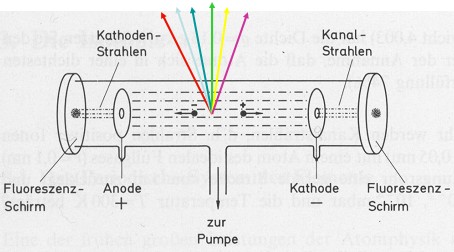
\includegraphics[width=\textwidth]{fig/3-SpektroskopieGasentladung.png}
	\caption{Spektroskopie von Gasentladungen}
\end{figure}

Man bringt in eine Gasröhre Elektroden ein, an die man eine hohe Spannung
anlegt. Es kommt zur Gasentladung, ein Lichtbogen wird beobachtet.
Spektroskopiert man den Lichtbogen, wird kein kontinuierliches Spektrum
festgestellt, sondern lediglich wenige diskrete Frequenzen.\bsphere
\end{bspn}

%TODO: Experiment Reflexion am Gitter
%TODO: Experiment Absorptionsspektroskopie
%TODO: Experiment Laserspektroskopie, Lösung des Dopplereffekts

Bei Spektroskopie steht die Frequenzmessung im Mittelpunkt. Die Präzession
dieser Messung ist heute auch im optischen Frequenzbereich so groß, dass man
mithilfe von optischen Frequenzmessungen Uhren bauen kann, die Zeit so exakt
messen, wie Cäsium Uhren, welche ebenfalls auf einer Mikrowellenfrequenzmessung
basiert. Es wird daher diskutiert, ob die Definition der Sekunde durch eine
optische Übergangsfrequenz gegeben werden soll.

 \begin{figure}[!htbp]
	\centering
	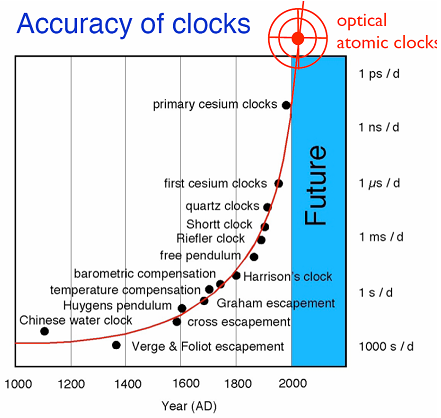
\includegraphics[width=\textwidth]{fig/3-AccuracyOfClocks.png}
	\caption{Präzission von Atomuhren.}
\end{figure}

Die Frequenz ist aber auch im Alltag eine sehr wichtige Messgröße.
\begin{bspn}
GPS basiert auf Längenmessungen, die man durch Laufzeitmessungen der GPS
Signale realisiert,
\begin{align*}
s = v\cdot t = c\cdot\frac{1}{f}.
\end{align*}
Je genauer die Frequenz bestimmt ist, desto genauer ist die
Positionsbestimmung.\bsphere
\end{bspn}


\subsection{Bohr'sches Atommodell}

Niels Bohr\footnote{Niels Henrik David Bohr (* 7. Oktober 1885 in Kopenhagen; †
18. November 1962 in Kopenhagen) war ein dänischer Physiker und
Nobelpreisträger für Physik des Jahres 1922} stellte 1913 erstmals
das später nach ihm benannte Atommodell vor.

Er suchte nach Erklärungen für den experimentellen Befund, dass
Atomspektren aus diskreten Linien bestehen.

Im sichtbaren Bereich kannte man die Balmer-Serie\footnote{Johann Jakob Balmer
(* 1. Mai 1825 in Lausen, Kanton Basel-Landschaft; † 12. März 1898 in Basel)
war ein Schweizer Mathematiker und Physiker.} (1885, $n'=2$) mit,
\begin{align*}
&\lambda = \frac{n^2}{n^2-2^2}G,\qquad m>2,\ B=364.56\mathrm{nm}\\
&\overline{\nu} = \frac{1}{\lambda} = R\left(\frac{1}{2^2}-\frac{1}{n^2}
\right),
\end{align*}
wobei $\overline{\nu}$ die \emph{Wellenzahl} und $R$ die empirisch bestimmte
\emph{Rydbergkonstante} bezeichnen. Im Ultravioletten die
Lyman-Serie\footnote{Theodore Lyman (* 23. November 1874 in Boston,
Massachusetts; † 11. Oktober 1954 in Cambridge, Massachusetts) war ein
amerikanischer Physiker.} (1906, $n'=1$), im Infraroten die
Paschen-Serie\footnote{Friedrich Paschen (* 22. Januar 1865 in Schwerin; † 25.
Februar 1947 in Potsdam) war ein deutscher Physiker, der 1921 gemeinsam mit
Ernst Back den Paschen-Back-Effekt entdeckte.} (1908, $n'=3$) und die
Brackett-Serie\footnote{Frederick Sumner Brackett (* 1. August 1896 in
Claremont, California; † 28. Januar 1988) war ein US-amerikanischer Physiker
und Spektroskopiker.} (1923, $n'=4$). \begin{figure}[!htbp]
	\centering
	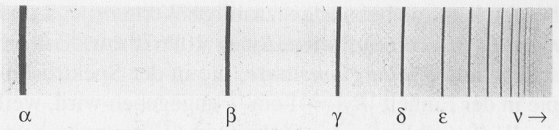
\includegraphics[width=\textwidth]{fig/3-BalmerSerie.png}
	\caption{Balmer Serie 1885}
\end{figure}

Als empirisches Ergebnis wurde 1913 von Rydberg\footnote{Johannes Robert
Rydberg (* 8. November 1854 in Halmstad; † 28. Dezember 1919 in Lund) auch
bekannt als Janne Rydberg, war ein schwedischer Physiker.} postuliert,
\begin{align*}
\overline{\nu} = R\left(\frac{1}{{n'}^2}-\frac{1}{n^2}\right),\quad n'<n\in\N.
\end{align*}

Bohr kannte bereits das Rutherford'sche Atommodell, bei dem ein Elektron um den
Kern in der Mitte kreist. Die Elektrodynamik verlangt jedoch, dass das auf die
Kreisbahn gezwungene Elektron kontinuierlich Energie abstrahlt und somit
zwangsläufig in den Kern stürzt.
%TODO: Skizze Spiralbahn

Um dieses Problem zu lösen, stellte Bohr folgende Postulate auf.
\begin{enumerate}[label=\arabic{*})]
  \item Das Atom ähnelt einem Planetensystem (Rutherford), bei dem die
  Elektronen um den Kern kreisen.
  \item Die Coulomb-Wechselwirkung zwischen Kern und Elektron und die 
  Zentrifugalkraft kompensieren sich.
  \item Es sind nur bestimmte Energieniveaus zulässig.
  \item Die Bewegung der Elektronen erfolgt strahlungslos.
  \item Die Elektronen können jedoch zwischen den erlaubten Energieniveaus
  springen und emittieren dabei Photonen mit
\begin{align*}
\nu = \frac{\Delta E}{h} = \frac{E_n-E_{n'}}{h},\quad \text{Planck (1900)}.
\end{align*}
\item \textit{Korrespondenzprinzip}. Für große $n$, also große Bahnradien,
sollen die klassischen Gesetze gelten.
\end{enumerate}

\begin{figure}[!htbp]
	\centering
	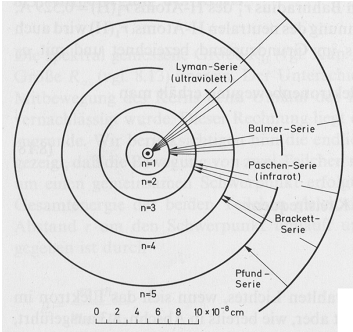
\includegraphics[width=\textwidth]{fig/3-BohrscherWasserstoff.png}
\end{figure}


Wir wollen diese Postulate nun mathematisch erfassen. Zentripetal- und
Coulombkraft sind im Gleichgewicht,
\begin{align*}
&F_{\text{Coulomb}} = -\frac{1}{4\pi\ep_0}\frac{Ze^2}{r^2},\quad
F_{\text{Zentripetal}} = mr\omega^2\\
&F_{\text{Zentripetal}}+F_{\text{Coulomb}} = 0.
\end{align*}
Dies ergibt eine Kreisbahn für das Elektron mit,
\begin{align*}
&\frac{1}{4\pi\ep_0}\frac{Ze^2}{r^2} = mr\omega^2\tag{1}\\
\Rightarrow\;&r(\omega) =
\left(\frac{1}{4\pi\ep_0}\frac{Ze^2}{m\omega^2}\right)^{1/3}\tag{2}.
\end{align*}
Betrachtet man nun die Energiewerte,
\begin{align*}
&E = E_{\text{kin}} + E_{\text{pot}}\\
&E_{\text{kin}} = \frac{1}{2}mv^2 = \frac{1}{2}mr^2\omega^2\\
&E_{\text{pot}} = \frac{1}{4\pi\ep_0}\int\limits_{\infty}^r
\frac{Ze^2}{{r'}^2}\dr' = -\frac{1}{4\pi\ep_0}\frac{Ze^2}{r}\\
\Rightarrow & E = \frac{1}{2}mr^2\omega^2 - \frac{1}{4\pi\ep_0}\frac{Ze^2}{r}
\end{align*}
Setzen wir nun unsere Ausdrücke für $E_{\text{pot}}$ und $r(\omega)$ ein,
\begin{align*}
\overset{(1)}{\Leftrightarrow} & E = \frac{1}{2}mr^2\omega^2 - mr^2\omega^2 =
-\frac{1}{2}mr^2\omega^2 \overset{(2)}{=}
-\frac{1}{2}m\left(\frac{1}{4\pi\ep_0}\frac{Ze^2}{m\omega^2}\right)^{2/3}\omega^2\\
&\quad 
= -\frac{1}{2}\left(\frac{1}{(4\pi\ep_0)^2}m\omega^2Z^2e^4\right)^{1/3},\tag{3}
\end{align*}
und verwenden Bohrs Postulat der diskreten Energieniveaus,
\begin{align*}
&E_n = -R\frac{hc}{n^2},\qquad n,n'=1,2,3,\ldots\text{ Quantenzahlen}\\
&E_{n'} = -R\frac{hc}{{n'}^2},\\
\Rightarrow & \Delta E = E_n-E_{n'} =
Rhc\left(\frac{1}{{n'}^2}-\frac{1}{n^2}\right).
\end{align*}
Das Modell erklärt somit das empirische Ergebnis,
\begin{align*}
\nu = \frac{\Delta E}{h} = Rc\left(\frac{1}{{n'}^2}-\frac{1}{n^2}\right),\quad
\nu = c\overline{\nu}.
\end{align*}
Betrachten wir $\Delta E$ für $n-n'=1$, so ergibt sich,
\begin{align*}
\nu = Rc\left(\frac{1}{(n-1)^2}-\frac{1}{n^2}\right) = 
Rc\frac{1}{n^2}\left(\frac{1}{\left(1-\frac{1}{n}\right)^2}-1\right).\tag{4}
\end{align*}
Für die Eigenenergien erhalten wir die Beziehung,
\begin{align*}
E_n = -\frac{1}{2}\left(\frac{1}{(4\pi\ep_0)^2}Z^2e^4m\omega^2\right)^{1/3} =
-\frac{Rhc}{n^2}.\tag{5}
\end{align*}
Klassisch erwarten wir so (Auflösen von (5) nach $\omega$),
\begin{align*}
\nu_{\text{klass.}} = \frac{\omega}{2\pi} \sim \frac{1}{n^3}.
\end{align*}
In Gleichung (4) haben wir jedoch $\sim\frac{1}{n^2}$.

Beachten wir, dass Bohrs Postulate nur für große $n$ eine Übereinstimmung
besagen, müssen wir den zweiten Faktor in (4) entwickeln,
\begin{align*} 
\frac{1}{\left(1-\frac{1}{n}\right)^2}
\approx 1 + \frac{2}{n} + \frac{3}{n^2}+\ldots
\end{align*}
Wenden wir diese Entwicklung in (4) an, so ergibt sich
\begin{align*}
\nu = Rc\frac{2}{n^3},\tag{6}
\end{align*}
was wieder mit der klassischen Erwartung übereinstimmt.

Wir wollen nun diesen Zusammenhang nutzen, um die Rydbergkonstante $R$ konkret
zu berechnen,
\begin{align*}
&\frac{Rhc}{n^2} = \frac{1}{2}\left(\frac{1}{(4\pi\ep_0)^2}Z^2e^4m\omega^2
\right)^{1/3} \overset{(6)}{=}
\frac{1}{2}\left(\frac{1}{(4\pi\ep_0)^2}Z^2e^4m\left(2\pi \frac{2Rc}{n^3}\right)^2
\right)^{1/3}.
\end{align*}
Für Wasserstoff erhalten wir so den Wert,
\begin{align*}
R = \frac{me^4}{8\ep_0^2 h^3 c}.\tag{7}
\end{align*}
Für Messung und Rechnung ergibt sich der Unterschied,
\begin{align*}
&R_{\text{Messung}} = (109737.318\pm 0.012)\mathrm{cm^{-1}},\\
&R_{\text{Rechnung}} = (109677.581)\mathrm{cm^{-1}}.
\end{align*}
Wir sehen, dass die Rechnung eine große Übereinstimmung mit den experimentellen
Daten hat.

Später werden wir diese Vorhersage noch verbessern, indem wir mit der
reduzierten Masse rechnen, da der Kern nicht - wie angenommen - unendlich
schwer ist und sich in Ruhe befindet, sondern sich mitbewegt.

\begin{bspn}
Der Bohrradius der ``kleinsten Bahn'' ($n=1$) im Wasserstoff-Atom ist
\begin{align*}
a_0 = 0.529 \AA,\qquad \AA = 10^{-10}\mathrm{m}.\bsphere
\end{align*}
\end{bspn}

Betrachten wir den Drehimpuls $\vec{l} = \vec{r}\times\vec{p}$ im Bohr'schen
Atommodell des Wasserstoffatoms, so ergibt sich,
\begin{align*}
\abs{\vec{l}} &= mr_n^2\omega_n \overset{(2)}{=}
m\left(\frac{1}{4\pi\ep_0}\frac{e^2}{m\omega_n^2}\right)^{2/3}\omega_n\\
&\overset{(6)}{=} m\left(\frac{1}{4\pi\ep_0}\frac{e^2}{m}\right)^{2/3}
\left(\frac{n^3}{4\pi R c}\right)^{1/3}
=\left(\frac{1}{(2\pi)^3}\frac{me^4}{8\ep_0^2h^3c}\frac{1}{R} \right)^{1/3}nh
 \\
&= n\hbar.
\end{align*}
Der Drehimpuls steigt also linear mit der Hauptquantenzahl an. Im Grundzustand
($n=1$) ist $\abs{\vec{l}}=\hbar$.
\begin{bemn}
Bohr und Sommerfeld haben diese Erkenntnisse genutzt, um eine allgemeine
Quantisierungsbedingung für geschlossene Bahnen aufzustellen,
\begin{align*}
\oint \vec{p} \dvecr =n h,
\end{align*}
die \emph{Bohr-Sommerfeldsche-Quantisierungsmethode}.
Ausgehend von dieser Quantisierung lassen sich andere Größen besonders
geschickt quantisieren. In Potentialen mit geschlossenen Bahnkurven ist
dies daher eine sehr gute Grundlage.
Dennoch hat sie ihre Grenzen. Das freie Teilchen wird beispielsweise von dieser
Methode nicht erfasst, da es keine geschlossene Bahnkurve besitzt. Später werden wir diese,
heute als antiquiert geltende Methode, durch die Schrödingergleichung ersetzen, 
mit der uns ein allgemeiner Ansatz für beliebige Potentiale zur Verfügung
steht.\maphere
\end{bemn}

Für die Umlauffrequenz erhalten wir den Wert,
\begin{align*}
\omega_n = \frac{4\pi Rc}{n^3} =
\frac{1}{(4\pi\ep_0)^2}\frac{Z^2e^4m}{\hbar^3n^3}.
\end{align*}
\begin{bspn}
Die Umlauffrequenz des Wasserstoffatoms im Grundzustand $(Z=1,n=1)$ ist
\begin{align*}
\omega(H) \approx 10^{16}\mathrm{s}^{-1}.\bsphere
\end{align*}
\end{bspn}

Die Geschwindigkeit des Elektrons auf der Bohrschen Bahn ist,
\begin{align*}
v = \omega_n r_n = Z\underbrace{\frac{e^2}{4\pi\ep_0\hbar
c}}_{\alpha}\frac{1}{n}c,\quad
\alpha\approx\frac{1}{137}\text{ heißt \emph{Feinstrukturkonstante}}.
\end{align*}
Die Geschwindigkeit ist zwar groß, beim Wasserstoffatom jedoch noch hinreichend
klein, um ohne relativistische Rechung auszukommen. Für größere Ordnungszahlen
muss man jedoch relativistische Effekte berücksichtigen.

Für Atome mit $Z\approx 137$ ist $v\approx c$ und das Modell bricht zusammen.
Die ``stationären Bahnen'' sind dann nicht mehr stationär, die Atome sind
nicht mehr stabil, sie zerfallen.

Die Bindungsenergie ist gegeben durch,
\begin{align*}
E_n = -\frac{Rhc}{n^2}= -\frac{1}{2}m\omega_n^2r_n^2 =
-\frac{Z^2e^4m}{32\pi^2\ep_0^2\hbar^2}\frac{1}{n^2}.
\end{align*}

\begin{bspn}
Für $Z=1,n=1$ erhalten wir
\begin{align*}
E_n = -13.6\mathrm{eV},
\end{align*}
was ebenfalls sehr gut mit der experimentellen Erfahrung übereinstimmt.\bsphere
\end{bspn}

\textit{1. Bewährungsprobe des Bohrschen Modells.}
\begin{align*}
\Delta R = R_{\text{exp}}-R_{\text{theo}} = -60\mathrm{cm^{-1}}\qquad
(H\text{-Atom})
\end{align*}
Wir wollen nun die Mitbewegung des Kerns berücksichtigen und rechnen mit der
reduzierten Masse,
\begin{align*}
\mu = \frac{m_em_{\text{Kern}}}{m_e+m_{\text{Kern}}}
= \frac{m_e}{1+\frac{m_e}{m_{\text{Kern}}}}
\end{align*}
%TODO: Bild Schwerpunktsystem
Die Rydbergkonstante errechnet sich somit durch,
\begin{align*}
R_\mu = \frac{\mu e^4}{8\ep_0^2 h^3c} =
\frac{1}{1+\frac{m_e}{m_{\text{Kern}}}}R_\infty.
\end{align*}
Als Abweichung vom gemessenen Wert der Rydbergkonstante erhalten wir nun,
\begin{align*}
\Delta R = -59\mathrm{cm^{-1}}\qquad (H\text{-Atom}),
\end{align*}
d.h. durch die Berücksichtigung der Mitbewegung des Kerns erhalten wir eine
etwas höhere Genauigkeit.

Als Anwendung können wir unter Annahme des Bohrschen Atommodells 
das Verhältnis von Protonen und Elektronenmasse bestimmen,
\begin{align*}
\frac{m_p}{m_e} = 1836.15,
\end{align*}
was ebenfalls sehr gut mit den massenspektrometrischen Messungen übereinstimmt.

Wenn wir vom Wasserstoff zum nächst schwereren Isotop dem Deuterium übergehen
(Isotopieverschiebung), ergibt sich
\begin{align*}
&R_H = 109677.581\mathrm{cm^{-1}},\\
&R_D = 109670.7\mathrm{cm^{-1}},
\end{align*}
in sehr guter Übereinstimmung mit den Messergebnissen.

\sfigure%
	{3-KorrekturMitbewegungKern.pdf}%
	{\HakenWolf, S. 110}%
	{Energiekorrektur wegen Mitbewegung des Kerns für die Rydberkonstante einiger
	Einelektronen Atome.}
% \begin{figure}[!htbp]
% 	\centering
% 	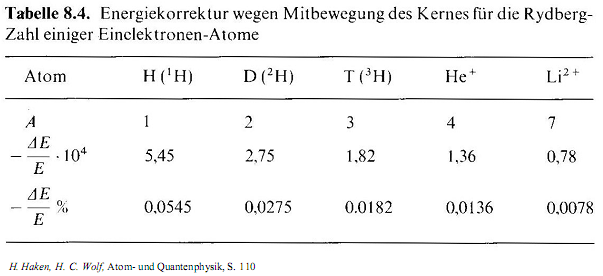
\includegraphics[width=\textwidth]{fig/3-KorrekturMitbewegungKern.png}
% \end{figure}

\textit{2. Bewährungsprobe des Bohrschen Modells.}

Für Atome mit höherer Ordnungszahl aber nur einem Elektron,
d.h. $He^+$, $Li^{++}$, $Be^{+++}$, usw. erhalten wir ein Wasserstoff ähnliches
Spektrum. Das Bohr-Sommerfeld-Modell sagt für die Bindungsenergie
\begin{align*}
E_n \sim \frac{Z^2}{n^2},
\end{align*}
voraus, d.h. sie steigt quadratisch mit $Z$ an. Auch dies lässt sich experimentell
bestätigen. Ein Extremfall in guter Übereinstimmung ist $U^{91+}$.

\subsubsection{Erweiterung des Bohr'schen Atommodells nach Sommerfeld}

Lässt man nicht nur Kreis- sondern auch Ellipsenbahnen zu, kann man das Modell
zum \emph{Bohr-Sommerfeld-Atommodell} erweitern. Die Ellipsengleichung ist
\begin{align*}
r = \frac{a(1-\ep^2)}{1+\ep\cos\ph},
\end{align*}
mit der goßen Halbachsen $a$ und der Exzentrität $\ep$.
\begin{figure}[!htpb]
\centering
\begin{pspicture}(0,-0.64)(2.4,0.64)
\psellipse(1.2,0.0)(1.2,0.64)
\psline(1.2,0.0)(1.2,0.62)
\psline(1.2,0.0)(2.38,0.0)

\rput(1.05,0.305){\color{gdarkgray}$b$}
\rput(1.82,-0.115){\color{gdarkgray}$a$}
\end{pspicture}\qquad
\begin{pspicture}(-0.2,-0.7)(2.2,0.6)
\pscircle(0.33,0.16){0.33}
\psellipse(1.55,0.14)(0.55,0.07)

\rput(0.31,-0.365){\color{gdarkgray}$\ep=0$}
\rput(1.53,-0.365){\color{gdarkgray}$\ep\to1$}
\end{pspicture} 
\caption{Ellipse mit großer Halbachse $a$ und kleiner Halbachse $b$ (links)
Einfluss der Exzentrität (rechts).}
\end{figure}
Eine Ellipsenbahn hat kleineren Drehimpuls als eine Kreisbahn.  Für $\ep=0$ 
erhalten wir den Kreis zurück, divergiert die Exzentrität $\ep\to1$, so
pendelt das Elektron durch den Kern $\Rightarrow l=0$.

Um dies herzuleiten, wählt man eine Bindungsenergie und eine
Quantisierungsbedingung und löst das Keplerproblem. Die Bindungsenergie ist
\begin{align*}
E_n = -\frac{Ze^2}{2a} = -\frac{Rhc}{n^2},
\end{align*}
hängt also nicht von $\ep$ ab. Es sind somit nicht nur Kreisbahnen als Lösungen
zugelassen sondern auch Ellipsen. Klassisch sind alle Bahnen mit $\ep\in[0,1)$
erlaubt, die quantenmechanische Behandlung nach Sommerfeld fordert jedoch,
\begin{align*}
&\oint p(r)\dr = n_r h,\\
&\oint p(\ph)\dph = n_\ph h.
\end{align*}
D.h. es sind nur diskrete $\ep$ erlaubt. Wir sehen wie in der Kernphysik, dass
für hohe Quantenzahlen, die Zustände zunehmend entarten, d.h. unterschiedliche
Zustände die gleiche Energie haben.

\begin{figure}[!htbp]
\centering
\begin{pspicture}(-0.5,-2.12)(4.2,2.3)
\psline{->}(0.74,-1.8)(0.74,2.08)
\psline(1.12,-1.6)(1.36,-1.6)
\psline(1.12,0.18)(1.36,0.18)
\psline(1.12,0.98)(1.36,0.98)
\psline(1.12,1.38)(1.36,1.38)
\psline(1.72,0.18)(1.96,0.18)
\psline(1.72,0.98)(1.96,0.98)
\psline(1.72,1.38)(1.96,1.38)
\psline(2.34,0.98)(2.58,0.98)
\psline(2.34,1.38)(2.58,1.38)
\psline(2.92,1.38)(3.16,1.38)
\psline(0.6152487,-1.6)(0.76,-1.6)
\psline(0.6152487,0.18)(0.76,0.18)
\psline(0.6152487,0.98)(0.76,0.98)
\psline(0.6152487,1.38)(0.76,1.38)

\rput[r](0.35,-1.615){\color{gdarkgray}$n=1$}
\rput[r](0.35,0.185){\color{gdarkgray}$n=2$}
\rput[r](0.35,0.965){\color{gdarkgray}$n=3$}
\rput[r](0.35,1.385){\color{gdarkgray}$n=4$}
\rput[r](0.45,2.08){\color{gdarkgray}$E$}

\rput(1.25,1.885){\color{gdarkgray}$1$}
\rput(1.85,1.885){\color{gdarkgray}$2$}
\rput(2.48,1.885){\color{gdarkgray}$3$}
\rput(3.07,1.885){\color{gdarkgray}$4$}

\rput(3.77,1.885){\color{gdarkgray}$n_r$}

\rput[b](1.25,-1.895){\color{gdarkgray}$s$}
\rput[b](1.87,-1.895){\color{gdarkgray}$p$}
\rput[b](2.43,-1.895){\color{gdarkgray}$d$}
\rput[b](3.07,-1.895){\color{gdarkgray}$f$}

\psline{->}(3.54,1.7)(4.12,1.7)
\end{pspicture} 
\caption{Entartung der Zustände $s$-sharp, $p$-principal, $d$-diffuse,
$f$-fundamental.}
\end{figure}

\textit{Bewährungsprobe für das Bohr-Sommerfeld-Modell.}

Betrachten wir die Spektrallinien des $H$-Atoms unter großer Auflösung,
sehen wir, dass die Linien aufgespalten sind, d.h. es sind nicht nur eine
sondern mehrere Linien sichtbar, die Entartung ist also (teilweise) aufgehoben.

Dies rührt daher, dass auf der Ellipsenbahn die Geschwindigkeit mit abnehmendem
Kernabstand zunimmt. Daher sind in Kernnähe große Geschwindigkeiten möglich
und relativistische Korrekturen notwendig.  Durch die relativistische
Massenzunahme wird die Energie abgesenkt und daher die Entartung der Zustände
aufgehoben.

\sfigure[H]%
	{3-TermschemaWasserstoff.pdf}%
	{\DemtroederThree, S. 172}%
	{Vollständiges Termschema des H-Atoms unter Berücksichtigung verschiedener 
	Wechselwirkungen. Die Fein- und die Hyperfeinstruktur und die
	Lamb-Verschiebung sind nicht maßstabsgetreu gezeichnet.}

Durch die Quantisierung der Exzentrizität erhalten wir neben der Quantisierung
des Bahndrehimpulses einen weiteren Freiheitsgrad. Durch die notwendigen
relativistischen Korrekturen lässt sich die sog. Feinstrukturaufspaltung
beschreiben.

Nun sind die Keplerbahnen nicht nur auf die Äquatorialebene beschränkt sondern
können sich beliebig im Raum orientieren. Jedoch ist auch diese Orientierung
quantisiert, was zu einem dritten Freiheitsgrad führt. In Polarkoordinaten
lautet daher unsere Quantisierungsbedingung,
\begin{align*}
\oint p_r \dr = n_r h,\\
\oint p_\th \dr = n_\th h,\\
\oint p_\psi \dr = n_\psi h,
\end{align*}
was zu einer weiteren Entartung führt. In externen Magnetfeldern wird diese
Entartung aufgehoben (\emph{Zeeman-Effekt}).

\subsubsection{Zusammenfassung}

Das Bohr-Sommerfeld-Modell kann sehr viele Erfolge verzeichnen:
\begin{itemize}
  \item Spektrallinien und Rydbergkonstante,
  \item Isotopieverschiebung ($H$-ähnliche Atome),
  \item Feinstrukturaufspaltung (Sommerfeld),
  \item Ansatzweise Zeemaneffekt (Verhalten von $H$-Atom im Magnetfeld).
\end{itemize}

Jedoch treten bei der Beschreibung mittels diesem Modell auch zahlreiche
Probleme auf:
\begin{itemize}
  \item Physikalische Erklärung für die stabilen Zustände fehlt.
  \item Beschreibung des freien Elektrons ist nicht möglich, da dessen
  Bahnkurve nicht geschlossen ist. Für nicht geschlossene Bahnen haben wir
  jedoch keine Handhabe, da wir die klassischen Gesetze außer Kraft gesetzt
  haben, um die Sprünge zu erklären.
  \item Linienstärken im Spektrum sind nicht vorhersagbar.
  \item Mehrelektronenatome $He$, $Li$, usw. können nicht erklärt werden, da
  das Modell bei mehr als einem Elektron versagt.
\end{itemize}

Indem wir das Bohr-Sommerfeld-Atommodell durch die Schrödingergleichung
ersetzen können wir diese und viele weitere Probleme lösen.

\subsection{H-Atom á la Schrödinger}

Wir wollen unser Modell nun weiterentwickeln. Eine wichtige Erkenntniss
lieferte De-Broglie\footnote{Louis-Victor Pierre Raymond de Broglie (* 15.
August 1892 in Dieppe, Normandie; † 19. März 1987 in Louveciennes, Département
Yvelines) war ein französischer Physiker und Nobelpreisträger für Physik des
Jahres 1929.} 1924, als er die Welleneigenschaften der Materie postulierte. In
seiner berühmt gewordenen Dissertation stellte er folgende Hypothesen auf:
\begin{enumerate}[label=(\roman{*})]
  \item Materie hat Welleneigenschaften.
  \item Klassische Punktteilchen ergeben sich durch Wellenpakete mit
  verschwindender Ausdehnung $\Delta x \to 0$.
  \item Die klassische Bahn entspricht dem Weg des Schwerpunkts des
  Wellenpakets.
\end{enumerate}
Daraus ergibt sich für die Gruppengeschwindigkeit der Materiewelle
\begin{align*}
v_g = \frac{\partial \omega}{\partial k} \overset{!}{=} \frac{p}{m},
\end{align*}
da sie mit der Geschwindigkeit des klassischen Teilchens übereinstimmen muss.
Mit $\omega = \frac{\hbar k^2}{2m}$ folgt somit,
\begin{align*}
&v_g = \frac{\hbar k}{m}\\
\Rightarrow & p = \hbar k,\quad \lambda_\text{dB} = \frac{h}{p}.
\end{align*}
Mit der De-Broglie-Wellenlänge $\lambda_\text{dB}$.

1927 wurde der Wellencharakter von Elektronen durch die Beugung eines
Elektronenstrahls an einem Kristall schließlich experimentell nachgewiesen.

1991 gelang auch die Streuung von He-Atomen an einem Doppelspalt.
\sfigure%
	{3-HeliumDoppelspalt.pdf}
	{}
	{Young'scher Doppelspaltversuch mit Helium}
Jedes He-Atom wird auf dem Schirm zwar als Punkt mit ($x,y$)-Koordinaten
erkannt, die Wahrscheinlichkeitsverteilung entspricht jedoch einem
Doppelspalt Beugungsmuster. Da sich stets höchstens ein Atom in der
Versuchsappartur befand, müssen die He-Atome mit sich selbst
interferieren.

\sfigure[H][0.7]%
	{3-HeliumDoppelspaltMessung.pdf}
	{}
	{Auftreffende Heliumatome auf dem Schirm nach passieren des 
	Doppelspalts.}
	
	 Jedes Atom trifft als lokalisiertes Teilchen auf dem Schirm auf.
	Mit zunehmender Dauer des Experiments erkennt man die
	Wahrscheinlichkeitsverteilung der Atome, welche der quantenmechanischen
	Erwartung aufgrund der Welleneigenschaften der Materie folgt.

Aufgrund der endlichen Ausdehnung des Eintrittsspaltes kommt es zum leichten
``verschmieren'', weshalb kein ``perfektes Minimum'' (Wsk $= 0$) zu erkennen
ist, sondern lediglich eine kleinere Auftreffwahrscheinlichkeit.

\subsubsection{Naives Modell der Wellennatur des Elektrons}
Bevor wir zur Schrödingergleichung übergehen, wollen wir noch ein naives Modell
zur Wellennatur des Elektrons auf Basis des
Bohr-Sommerfeld-Atommodells entwickeln.
\begin{figure}[!htbp]
\centering
\begin{pspicture}(0,-1.03)(2.26,1.03)
\psdots[linecolor=darkblue](1.0,0.01)
\psarc[linecolor=yellow]{->}(1.01,0.0){1.01}{46.301952}{14.858615}
\psdots[linecolor=yellow](1.72,0.71)

\psline{<->}(1.08,0.07)(1.64,0.63)

\rput(2.08,0.815){\color{gdarkgray}$e^-$}
\rput(0.86,-0.28){\color{gdarkgray}$p^+$}
\rput(1.26,0.495){\color{gdarkgray}$r$}
\end{pspicture}
\caption{Naives Modell der Elektronenbewegung.}
\end{figure}

Das Elektron auf der Bahn wird durch eine bestimmte Wellenlänge
$\lambda_{\dB}$ beschrieben. Stationäre Zustände entsprechen nun stehenden
Wellen. Die Bedingung dafür ist
\begin{align*}
&2\pi r = n\lambda_{\dB},\qquad \lambda_{\dB} = \frac{h}{p},\\
\Rightarrow & \frac{2\pi r}{\lambda_{\dB}} = \frac{2\pi r}{h}p = n\\
\Rightarrow & \abs{\vec{l}} = rp = n\hbar.
\end{align*}
Mit dieser Vorstellung kann man die Quantisierungsbedinung für stationäre
Zustände
\begin{align*}
\oint p(x)\dx = n h
\end{align*}
erklären. Die Wellentheorie ist somit dem Bohr-Sommerfeld-Atommodell überlegen.

\subsubsection{Quantenmechanische Behandlung des H-Atoms á la Schrödinger}

Wir wollen nun zur Beschreibung der Elektronen als Materiewellen
mit Hilfe der Schrödingergleichung übergehen. Die allgemeine
zeitabhängige Schrödingergleichung hat die Form
\begin{align*}
i\hbar \partial_t \Psi = -\frac{\hbar^2}{2m}\nabla^2\Psi + V(r)\Psi.
\end{align*}
\begin{bemn}[Bemerkungen.]
\begin{enumerate}[label=\arabic{*}.)]
  \item Im Gegensatz zur Klassischen Mechanik beinhaltet die
  Schrödingergleichung keine 2. Zeitableitung. Das Anfangswertproblem ist daher
  bereits durch die Angabe von $\Psi(t=0)$ eindeutig lösbar, in der
  Klassischen Mechanik war stets auch der Anfangswert der Zeitableitung
  erforderlich. Das bedeutet für die Interpretation, dass $\Psi$ einen Zustand
  bereits vollständig charakterisiert.
  \item Die Lösungsfunktionen sind komplexwertig. In der Klassischen Mechanik
  sind alle Lösungsfunktionen reellwertig, da sie beobachtbar sein müssen. Die
  Lösungen $\Psi$ der Schrödingergleichung sind daher nicht für ein einzelnes
  Teilchen beobachtbar. Erst wenn wir zu 
\begin{align*}
\abs{\Psi}^2, \lin{\Psi^*\op{O}\Psi}, \ldots
\end{align*}
übergehen, erhalten wir beobachtbare Größen.
\item
Bisher hatten wir es stets mit Gleichungen zu tun, die wir aus Postulaten
ableiten konnten. Bei der Schrödingergleichung ist dies nicht der Fall,
da es (noch) kein tieferliegendes physikalisches Konzept gibt, das die
Schrödingergleichung ergibt.

Die Schrödingergleichung ist lediglich dadurch legitimiert, dass sie
funktioniert. Sie ist allerdings die am besten getestete Gleichung. Es gibt
(noch) kein Experiment im Geltungsbereich der nichtrelativistischen Quantenmechanik, das
einen Widerspruch zu ihr erzeugt. \maphere
\end{enumerate}
\end{bemn}


Wir wollen nun die Schrödingergleichung für die Bewegung des Elektrons im
Coulombpotential $V$ lösen. Dabei sind wir nur an stationären Lösungen
interessiert, man kann diese als stehenden Materiewellen interpretieren. Betrachtet man
beispielsweise eine schwingende Saite in der Klassischen Mechanik, so wird
die Energie die Schwingung durch die stationären Knoten charakterisiert.
Man kann auch das Elektron als ``eingespannt'' ansehen (im Coulombpotential).
Die stationären Lösungen charakterisieren die Bindungsenergie.

Das Coulomb-Potential ist kugelsymmetrisch, wir führen daher Kugelkoordinaten
ein, da hier $V$ nur von $r$ abhängt.
\begin{align*}
V(\vec{r}) = V(\abs{\vec{r}}) = V(r) = -\frac{e^2}{r}.
\end{align*}
Diese Symmetrie wird es uns ermöglichen,
die 3-dimensionale Schrödingergleichung in drei 1-dimensionale
Differentialgleichungen zu separieren. Wir sind dann in der Lage, eine
analytische Lösung zu berechnen. Im Gegensatz zum Bohr-Sommerfeld-Atommodell
erhalten wir also die vollständige Wellenfunktion und nicht nur die
Energieeigenwerte.

Um die Kugelsymmetrie auszunutzen, gehen wir nun zu Kugelkoordinaten über,
\begin{align*}
&r^2 = x^2+y^2+z^2,\\
&\cos\th = \frac{z}{r},\\
&\tan\ph = \frac{y}{r}.
\end{align*}
Der Laplace-Operator hat hier die Form,
\begin{align*}
\nabla^2 &= \left(\frac{\partial^2}{\partial x^2}+\frac{\partial^2}{\partial
y^2}+\frac{\partial^2}{\partial z^2}\right) = \ldots\\
&= \frac{1}{r}\frac{\partial}{\partial r}\left(r^2\frac{\partial}{\partial
r}\right) +
\frac{1}{r^2}\underbrace{\left[\frac{1}{\sin\th}\frac{\partial}{\partial\th}\left(\sin\th
\frac{\partial}{\partial\th}\right) +
\frac{1}{\sin^2\th}\frac{\partial^2}{\partial \ph^2}
\right]}_{-\frac{\op{l}^2}{\hbar^2}}\\
\op{H} &= -\frac{\hbar^2}{2m}\frac{1}{r^2}\frac{\partial}{\partial
r}\left(r^2\frac{\partial}{\partial r}\right)+\frac{\op{l}^2}{\hbar^2r^2} +
V(r).
\end{align*}
Für die Drehimpulsoperatoren gilt,
\begin{align*}
&\op{l} =\op{r}\times\op{p} = (\op{l}_x,\op{l}_y,\op{l}_z),\\
&\op{l}_x = \op{y}\op{p}_z - \op{z}\op{p}_y \mapsto i\hbar
\left(\sin\ph\frac{\partial}{\partial \th} +
\cos\th\cos\ph\frac{\partial}{\partial \ph}\right),\\
&\op{l}^2 \mapsto
-\hbar^2\frac{1}{r^2}\left[\frac{1}{\sin\th}\frac{\partial}{\partial\th}\left(\sin\th
\frac{\partial}{\partial\th}\right) +
\frac{1}{\sin^2\th}\frac{\partial^2}{\partial \ph^2}
\right].
\end{align*}
\begin{bemn}[Wichtige Beobachtungen.]
\begin{enumerate}[label=\arabic{*}.)]
  \item $\nrm{\op{l}_x,\op{l}_y} = i\hbar \op{l}_z$, 
  für alle zyklischen Permutationen von $x$, $y$ und $z$. Es ist also keine
  Richtung ist ausgezeichnet (Isotropie).
\begin{align*}
\Delta \op{l}_x \Delta \op{l}_y \ge \frac{\hbar}{2}\abs{\op{l}_z},
\end{align*}
d.h. nur eine Komponente kann gleichzeitig gemessen werden.
\item
$\nrm{\op{l}^2,\op{l}_x}=\nrm{\op{l}^2,\op{l}_x}=\nrm{\op{l}^2,\op{l}_x}=0$.
Das Betragsquadrat $\op{l}^2$ und eine Komponente (z.B. $\op{l}_z$) des
Drehimpulses sind gleichzeitig messbar.
\item $\nrm{\op{H},\op{l}^2}=\nrm{\op{H},\op{l}_z} = 0$. $\op{H}$,
$\op{l}^2$ und $\op{l}_z$ sind gleichzeitg messbar. Dies wird uns auf die
Quantenzahlen $(n,l,m)$ führen. Im Bohr-Sommerfeld-Modell hatten wir
$(n,n_\th,n_\ph)$.\maphere
\end{enumerate}
\end{bemn}
Wir wollen die Schrödingergleichung nun separieren.

\textit{0. Ansatz.} Wir sind an stationären Lösungen interessiert und gehen
daher zur zeitunabhängigen Schrödingergleichung über,
\begin{align*}
\underbrace{\left\{-\frac{\hbar^2}{2m}\nabla^2 + V(r)\right\}}_{\op{H}}\Psi(\vec{r})
= E\Psi(\vec{r}),
\end{align*}
wobei $E$ unsere Separationskonstante bezeichnet. Aufgrund der Separation von
Raum und Zeit erhalten wir den Ansatz,
\begin{align*}
\Psi(t,\vec{r}) = \Psi(\vec{r})e^{-\frac{iEt}{\hbar}}.
\end{align*}
Für jede Separation entsteht eine Separationskonstante, die jeweils eine
Quantenzahl entählt. Die Energie $E$ enthält die Hauptquantenzahl $n$.

\textit{1. Ansatz.} Separation in Radial- und Winkelanteil,
\begin{align*}
\Psi(r,\th,\ph) = R(r)Y(\th,\ph).
\end{align*}
$R(r)$ heißt \emph{Radialgleichung}. Zu ihr gehört die Differentialgleichung,
\begin{align*}
\frac{1}{R}\frac{\partial}{\partial r}\left(r^2 \frac{\diffd R}{\dr}\right) +
\frac{2mr^2}{\hbar^2}\left[E-V(r)\right] = l(l+1),
\end{align*}
mit der Separationskonstanten $l$.

\textit{2. Ansatz.}
\begin{align*}
Y(\th,\ph) = T(\th)\Phi(\ph).
\end{align*}
$\Phi(\ph)$ heißt \emph{Azimutalgleichung}. Die dazugehörige
Differentialgleichung ist
\begin{align*}
\frac{\partial^2\Phi}{\partial\ph^2} + m^2\Phi = 0,
\end{align*}
mit der Separationskonstanten $m$.\\
$T(\th)$ heißt \emph{Polargleichung}.
\begin{align*}
\frac{1}{T\sin\th}\frac{\partial}{\partial\th}\left(\sin\th
\frac{\partial T}{\partial\th}\right) + l(l+1) - \frac{m^2}{\sin^2\th} = 0.
\end{align*}

\subsubsection{Azimutalgleichung}
\label{subsubsec:Azimutalgleichung}

Dei einfachste Lösung besitzt die Azimutalgleichung, die wir als einzige
explizit lösen wollen. Da das System durch eine $2\pi$-Drehung in sich selbst übergeht,
ist es erforderlich, dass
\begin{align*}
\Phi_m(\ph+2\pi) = \Phi_m(\ph).
\end{align*}
Wir wählen daher als Ansatz
\begin{align*}
\Phi_m(\ph) = Ae^{im\ph},
\end{align*}
der für $m=0,\pm 1,\pm 2,\ldots$ bereits ein VONS bildet. Die
Aufenthaltswahrscheinlichkeit für eine $2\pi$-Integration ist $1$, es muss
also gelten,
\begin{align*}
&\int\limits_0^{2\pi} \abs{\Phi}^2\dph \overset{!}{=} 1\\
\Leftrightarrow & \abs{A}^2\int\limits_0^{2\pi}\abs{e^{im\ph}}^2\dph = 2\pi\\
\Rightarrow & A=\frac{1}{\sqrt{2\pi}}.
\end{align*}
Die Azimutale Lösung hat daher die Form,
\begin{align*}
\Phi_m(\ph) = \frac{1}{\sqrt{2\pi}}e^{im\ph},\qquad m\in\Z.
\end{align*}
$\Phi_m$ ist eine Eigenfunktion des Drehimpulsoperators $\op{l}_z$,
\begin{align*}
\op{l}_z\Phi_m = \hbar m\Phi_m,
\end{align*}
mit Eigenwert $\hbar m$, $m$ heißt \emph{Magnetquantenzahl}.

$\Phi_m$ ist ein Beispiel für eine komplexe quantenmechanische Größe.
Erst das Betragsquadrat $\abs{\Phi_m}^2$ ist beobachtbar.

Betrachten wir nur einen einzigen Zustand,
\begin{align*}
m = -1,0,1,\ldots
\end{align*}
so ist die Wahrscheinlichkeitsdichte homogen verteilt. Bei
Überlagerungszuständen wie beispielsweise
\begin{align*}
m_1 = 1,\quad m_2 = -1,\qquad \Phi_\text{ges} = \frac{1}{\sqrt{2}}\left(
\Phi_{m=+1} + \Phi_{m=-1} \right),
\end{align*}
wird die Wahrscheinlichkeitsdichte durch eine trigonometrische Funktion
beschrieben. Die Verteilung ist nicht mehr homogen, es treten Punkte auf
mit Aufenthaltswahrscheinlichkeit Null. Diese Punkte nennen wir \emph{Knoten}.

\subsubsection{Polargleichung}

Zur formalen Lösung der Polargleichung findet man in fast jedem einführenden
Quantenmechanik Werk eine ausführliche Rechnung. Für das Verständnis ist viel
mehr eine Interpretation der Lösung von Interesse.

Die Lösung der Polargleichung ist gegeben durch,
\begin{align*}
T_{lm}(\th) = N_{lm} P_{l}^m(\cos\th),
\end{align*}
$N_{lm}$ beschreibt einen Normierungsfaktor,
\begin{align*}
N_{lm} = \sqrt{\frac{2l+1}{2}\frac{(l-m)!}{(l+m)!}},
\end{align*}
$P_l^m(\cos\th)$ sind die zugeordneten Legendre Polynome.

\begin{bemn}
Die Winkelabhängigkeit $Y_{lm}(\th,\ph)=\Phi_m\cdot T_{lm}$ ist für alle
Zentralpotentiale gleich. Die Eigenfunktionen $Y_{lm}$ heißen
\emph{Kugelflächenfunktionen}.\maphere
\end{bemn}

\begin{figure}[!htbp]
	\centering
	\begin{align*}
    &P_{0}^{0}(\cos\th) = \frac{1}{2\sqrt{\pi}}\\
    &P_{1}^{1}(\cos\th) = -\frac{1}{2}\sqrt{\frac{3}{2\pi}}\sin\th\\
    &P_{1}^{0}(\cos\th) = \frac{1}{2}\sqrt{\frac{3}{2\pi}}\cos\th\\
    &P_{1}^{-1}(\cos\th) = +\frac{1}{2}\sqrt{\frac{3}{2\pi}}\sin\th\\
    &P_{2}^{2}(\cos\th) = +\frac{1}{4}\sqrt{\frac{15}{2\pi}}\sin^2\th\\
    &P_{2}^{1}(\cos\th) = -\frac{1}{2}\sqrt{\frac{15}{2\pi}}\sin\th\cos\th\\
    &P_{2}^{0}(\cos\th) = \frac{1}{4}\sqrt{\frac{5}{\pi}}(2\cos^2\th -
    \sin^2\th)\\
    &P_{2}^{-1}(\cos\th) = +\frac{1}{2}\sqrt{\frac{15}{2\pi}}\sin\th\cos\th\\
    &P_{2}^{-2}(\cos\th) = -\frac{1}{4}\sqrt{\frac{15}{2\pi}}\sin^2\th
    \end{align*}
	\caption{Zugeordnete Legendre Polynome $P_l^m$.}
\end{figure}

\begin{bspn} Für $m=0$ ist
$P_l^0(x) = P_l(x)$. Die $P_l(x)$ sind die Legendere Polynome,
\begin{align*}
&P_0(x) = 1,\quad
P_1(x) = x,\quad
P_2(x) = \frac{1}{2}(3x^2-1).\bsphere
\end{align*}
\end{bspn}
Eine Eigenschaft der Legendre Polynome ist, dass mit $l$ die Anzahl der
Nullstellen linear zunimmt. Darüber hinaus erhalten wir für gerades $l$ auch
gerade Funktionen und für ungerades $l$ ungerade Funktionen. Die Parität ist
daher gerade $(-1)^l$.

\begin{figure}[!htbp]
	\centering
	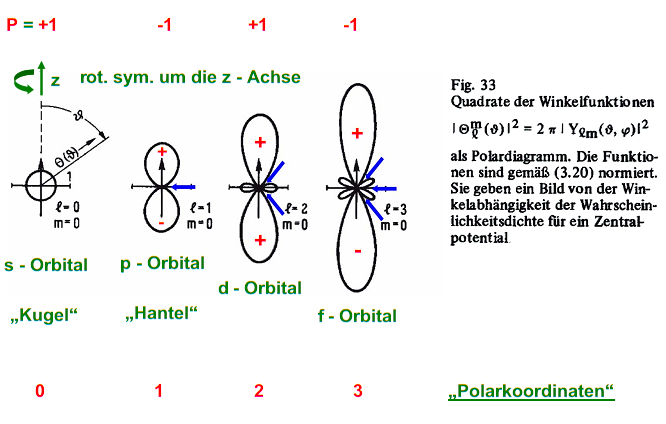
\includegraphics[width=\textwidth]{fig/3-KnotenPolarkoordinaten.png}
\end{figure}

Mit den Lösungen für $\Phi_m$ und $T_{lm}$ lassen sich die
$Y_{lm}$ angeben,
\begin{align*}
Y_{lm}(\th,\ph) = T_{lm}(\th)\Phi_m(\ph) = \frac{1}{\sqrt{2\pi}}
N_{lm}P_l^m(\cos\th)e^{im\ph}.
\end{align*}
Die Kugelflächenfunktionen $Y_{lm}$ sind die Eigenfunktionen zu $\op{l}^2$ und $\op{l}_z$,
\begin{align*}
&\op{l}^2Y_{lm} = \hbar (l+1)l Y_{lm}, && l=0,1,2,3,\ldots\\
&\op{l}_zY_{lm} = \hbar mY_{lm}, && \abs{m} \le l.
\end{align*}

Der Faktor $(l+1)$ kommt im Bohr'schen Atommodell nicht vor und folgt aus der
Wellennatur. Das bedeutet aber, dass der Drehimpulszustand nicht perfekt
gemessen werden kann, denn $\op{l}^2$ ist immer größer als $\op{l}_z^2$.
Selbst für maximales $m$, ($m=\pm l$) zeigt $\op{l}$ nicht exakt in
$z$-Richtung.

\begin{figure}[!htbp]
\centering
\begin{pspicture}(0,-1.67)(2.36,1.69)
\psline{->}(1.16,-1.65)(1.18,1.55)

\psellipse[linestyle=dashed,dashsep=0.06cm](1.18,-0.02)(1.18,0.33)
\psellipse[linestyle=dashed,dashsep=0.06cm](1.19,0.61)(0.97,0.26)
\psellipse[linestyle=dashed,dashsep=0.06cm](1.18,1.11)(0.68,0.2)
\psellipse[linestyle=dashed,dashsep=0.06cm](1.19,-0.65)(0.97,0.26)
\psellipse[linestyle=dashed,dashsep=0.06cm](1.18,-1.15)(0.68,0.2)

\psline[linecolor=darkblue]{->}(1.18,-0.03)(1.86,1.09)
\psline[linecolor=darkblue]{->}(1.18,-0.03)(2.16,0.59)
\psline[linecolor=darkblue]{->}(1.18,-0.03)(2.34,-0.03)
\psline[linecolor=darkblue]{->}(1.18,-0.01)(1.88,-1.17)
\psline[linecolor=darkblue]{->}(1.18,-0.01)(2.16,-0.67)

\rput[r](1.1,-0.025){\color{gdarkgray}\footnotesize$0$}
\rput[r](1.1,-1.165){\color{gdarkgray}\footnotesize$-2\hbar$}
\rput[r](1.1,-0.645){\color{gdarkgray}\footnotesize$-\hbar$}
\rput[r](1.1,0.595){\color{gdarkgray}\footnotesize$\hbar$}
\rput[r](1.1,1.095){\color{gdarkgray}\footnotesize$2\hbar$}
\rput(1.06,1.595){\color{gdarkgray}$z$}
\end{pspicture}
\caption{Mögliche Ausrichtung des Drehimpulses für $l=2$, $m=-2,-1,0,1,2$.}
\end{figure}

Für $m\neq 0$ haben die Kugelflächenfunktionen außerdem eine $(\sin\th)^m$
Abhängigkeit. Für $m\to\infty$ wird die Aufenthaltswahrscheinlichkeit jedoch in
die Äquatorialebene gedrückt, was wieder dem Korrespondenzprinzip entspricht.

Betrachtet man die räumliche Darstellung der Kugelflächenfunktionen, so sieht
man, dass die Quantenzahlen die Knotenflächen zählen. In den Knotenflächen ist
die Aufenthaltswahrscheinlichkeit Null.


\begin{figure}[H]
	\centering
	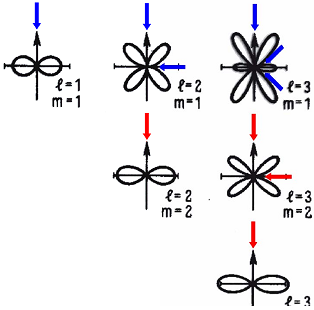
\includegraphics[width=0.5\textwidth]{fig/3-Kugelflaechenfunk.png}
	\caption{Knotenflächen der Kugelflächenfunktionen $\abs{Y_{lm}}^2$ in
	Abhängigkeit von $l$ und $m$.}
	%TODO: Mathematica
\end{figure}


\begin{figure}[!htbp]
	\centering
	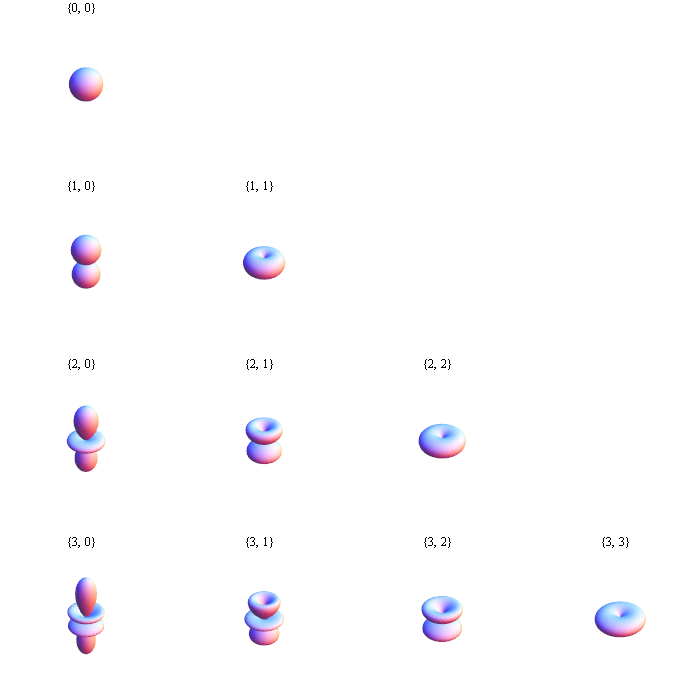
\includegraphics[width=0.8\textwidth]{fig/3-Kugelflaechenfunktionen.png}
	\caption{Graphische Darstellung zugeordneter Kugelflächenfunktionen.}
\end{figure}

%TODO: Bild Äquatorialdrehimpuls

%TODO: Bild Orbitale

\subsubsection{Radialgleichung}

Zur Lösung der Radialgleichung führen wir die Substitution $u = rR(r)$
durch.
\begin{align*}
\abs{u(r)}^2\dr = \abs{R(r)}^2r^2\dr
\end{align*}
beschreibt die Aufenthaltswahrscheinlichkeit des Elektrons in der Kugelschale
mit Radius $[r,r+\dr]$.

Die Gleichung nimmt nun eine uns bekannte Form an,
\begin{align*}
\frac{\diffd^2u}{\dr^2} + \frac{2m}{\hbar}\left[E-\underbrace{V(r) -
\frac{l(l+1)}{2mr^2}}_{V_{\text{Eff}}}\right]u = 0.
\end{align*}
Für die Energie erhalten wir so,
\begin{align*}
E_n = -\frac{R_\infty}{n^2},\qquad n=1,2,3,\ldots,\quad l\le n-1.
\end{align*}
Betrachtet man das effektive Potential, stellt man fest, dass für $l=0$ das
Elektron eine endliche Aufenthaltswahrscheinlichkeit im Kern hat. Es pendelt
quasi durch den Kern. Für $l>0$ wird die Potentialbarriere für abnehmendes $r$
immer größer, die Aufenthaltswahrscheinlichkeit im Kern ist Null.

\sfigure[H][0.8]%
	{3-EffektivesPotFuerRadial.pdf}
	{\KuckukAtom, S. 66}
	{Zum Zentrifugalpotential. a) Zustandekommen des effektiven Potentials, b,c)
	Wirkung der Potentialform auf die radiale Wellenfunktion $R(r)$.}
% 
% \begin{figure}[!htbp]
% 	\centering
% 	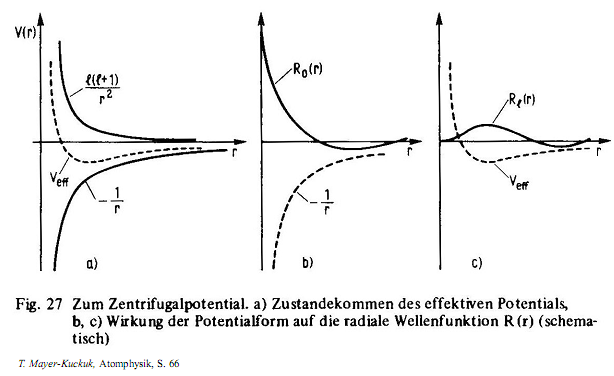
\includegraphics[width=\textwidth]{fig/3-EffektivesPotFuerRadial.png}
% \end{figure}

Betrachten wir Lösungen für $l=0$,
\begin{align*}
&R_{10}(\rho) =
2\left(\frac{Z}{a_0}\right)^{\frac{3}{2}} 1 \exp\left[-\frac{\rho}{2} \right],\\
&R_{20}(\rho) = \frac{1}{2\sqrt{2}}\left(\frac{Z}{a_0}\right)^{\frac{3}{2}}
(2-\rho) \exp\left[-\frac{\rho}{2} \right],\\
&R_{30}(\rho) = \frac{1}{9\sqrt{3}}\left(\frac{Z}{a_0}\right)^{\frac{3}{2}}
(6-6\rho-\rho^2) \exp\left[-\frac{\rho}{2} \right],
\end{align*}
mit $\rho = \frac{2Zr}{na_0}$, so werden diese durch die Laguerre-Polynome
beschrieben.

Erhöht man $l$ unter festem $n$, so verliert man bei jeder Erhöhung eine
Knotenfläche. Bei $l=n-1$ sind keine Knotenflächen mehr vorhanden.
$R_{nl}$ hat $(n-1)-l$ Nullstellen.

\sfigure[H][0.6]%
	{3-RadialteilWellenfunktion.pdf}
	{\HakenWolf, S. 171}
	{a) Die Wellenfunktion des Radialteils $R(r)$ des H-Atoms ist gegenüber der
	dimensionslosen Koordnate $\rho$ aufgetragen. Die an den Kurven angegebenen
	Indizes $(1,0)$, $(2,1)$, \ldots usw. entsprechen $(n,l)$, wobei $n$ die
	Hauptquantenzahl und $l$ die Drehimpulsquantenzahl. b) Die entsprechenden
	Aufenthaltswahrscheinlichkeiten in radialer Richtung. d.h. $4\pi \rho^2
	(\tilde{R}(\rho))^2$ sind gegenüber der dimensionslosen Koordinate $\rho$
	aufgetragen.}

\sfigure[H]%
	{3-EigenfunktionenDesWasserstoffatoms.pdf}
	{\KuckukAtom, S. 70}
	{Einige vollständige Eigenfunktionen des Wasserstoffatoms.}


\subsubsection{Anwendung der H-Atom Wellenfunktion}

Eine Schwäche des Bohr-Sommerfeld-Modells ist, dass man nicht vorhersagen
kann, wie wahrscheinlich ein Übergang zwischen zwei Energieniveaus ist und
daher die Lichtstärken im Spektrum des H-Atoms nicht erklären kann.

Wir wollen nun die Lösung der Schrödingergleichung für das H-Atom
interpretieren und dadurch einige Probleme des Bohr-Sommerfeld-Modells
lösen.

\begin{enumerate}[label=\arabic{*}.)]
\item Aufenthaltswahrscheinlichkeit des Elektrons im Kern.
\begin{align*}
l=0 \Rightarrow
\abs{\Psi_{n00}(r=0)}^2 = \abs{R_{n0}Y_{00}}^2 = \frac{Z^2}{\pi a_0^3n^3} \neq
0.
\end{align*}
D.h. wir haben eine endliche Aufenthaltswahrscheinlichkeit, die mit zunehmendem
$n$ abnimmt.
\begin{align*}
l>0\Rightarrow
\abs{\Psi_{nlm}(r=0)}^2 = \abs{R_{nl}Y_{lm}}^2 = 0,
\end{align*}
d.h. dass Elektronen mit $l>0$ keine Wechselwirkung mit einem punktförmigen Kern
haben.
\item Für den Erwartungswert des ``Bahnradius'' erhalten wir
\begin{align*}
\lin{r} = \int_{\R^3}\Psi^*r\Psi \dV = \frac{a_0}{2Z}\left((3n)^2 -l(l+1)
\right).
\end{align*}
$\lin{r}$ ist proportional zu $n^2$, was sich auch mit den Vorhersagen des
Bohr-Sommerfeld-Modell deckt. Für maximalen Drehimpuls $l=n-1$ und große
$n$ ist $l\approx n$ und daher
\begin{align*}
\lin{r} \sim \frac{a}{2Z}2n^2 = \frac{a}{Z}n^2,
\end{align*}
was gerade dem Radius der Kepplerbahn entspricht.

Für die Varianz erhalten wir,
\begin{align*}
&\lin{r^2}-\lin{r}^2 =
\begin{cases}
\frac{n^2(n^2+2)}{4Z^2} a_0^2, & \text{für }l=0,\\
\frac{n^2(2n+1)}{4Z^2} a_0^2, & \text{für }l=n-1,
\end{cases}\\
&\frac{(\Delta r)^2}{\lin{r}^2} =
\begin{cases}
\frac{1}{9}, & \text{für }l=0,\\
\frac{1}{2n}, & \text{für }l=n-1, 
\end{cases}
\end{align*}
d.h. die Unschärfe verschwindet für $n\to\infty$ und $l=n-1$, was gerade dem
Korrespondenzprinzip entspricht.

Für den Fall, dass alle Quantenzahlen groß werden,
\begin{align*}
n\to\infty,\quad l = n-1,\quad m=l,
\end{align*}
erhalten wir wieder die klassischen Kreisbahnen. Diese hoch angeregten Zustände
finden wir in \emph{zirkularen Rydbergatomen}.
\item Die Linienstärke im Spektrum ist proportional zur Wahrscheinlichkeit des
Dipolübergangs ($i$ - initial state, $f$ - final state)
\begin{align*}
\sim \abs{d_{i\to f}}^2 = \int_{\R^3} \Psi_f^* \op{d} \Psi_i \dV.
\end{align*}
Falls das Integral verschwindet, d.h. $\abs{d_{i\to f}}^2 = 0$ ist der Übergang
verboten und daher keine Linie im Spektrum sichtbar.

Wir wissen bereits, dass die Kugelflächenfunktionen den Winkelanteil der
Wellenfunktion des H-Atoms beschreiben und dass diese Eigenfunktionen des
Paritätsoperators sind. Wir können damit Auswahlregeln für optische
Übergange erarbeiten, denn damit $d_{if}\neq 0$ muss die Parität des
Integranden gerade sein, d.h. das Produkt von $\Psi_i$ und $\Psi_f$ muss
ungerade Parität haben. Die Partität der $Y_{lm}$ ist $(-1)^l$. Man kann
zeigen, dass nur Übergänge mit
\begin{align*}
&\Delta l = \pm 1
\end{align*}
erlaubt sind. Berücksichtigt man noch den Drehimpuls des Photons, das bei einem
optischen Übergang emittiert wird, erzwingt dies
\begin{align*}
\Delta m = 0,\pm 1.
\end{align*}
Das Bohr-Sommerfeld-Modell konnte dies nicht erklären. Die Übergänge wurden
lediglich postuliert (ohne physikalisches Verständnis). Jetzt können wir die
Übergänge erklären und quantifizieren. Ist $d_{i\to f}$ endlich, beginnt ein
Dipol bei der Übergangsfrequenz zu schwingen.
%TODO: l=0, l=1, usw. bildchen
Die Übergangsfrequenz ist viel höher als die Absorptions bzw. Emissionsrate, es
sind daher viele Oszillationen notwendig, bis der Übergang abgeschlossen ist.
Optische Übergänge entsprechen also Oszillationen hoher Güte. Die Dämpfung
durch die Abstrahlung ist dabei schwach. Die Anregungsenergie wird dabei in Form
von Photonen abgegeben.
\end{enumerate}

\newpage
\subsection{Drehimpuls und Spin}
\subsubsection{Klassische Betrachtung}
Klassisch betrachtet, bewegt sich das Elektron auf einer Kreisbahn um den Kern.
Damit ist ein Strom
\begin{align*}
I = \frac{a}{\tau} = -\frac{e}{T} = -\frac{ev}{2\pi r},
\end{align*}
verbunden, der die Fläche $A=\pi r^2$ umschließt.
\begin{figure}[!htbp]
\centering
\begin{pspicture}(0,-0.91411114)(1.94,0.91411114)

\psellipse[linestyle=dotted,dotsep=0.06cm](0.78,0.02)(0.78,0.32)
\psline{->}(1.42,0.2)(1.72,-0.02)
\psline[linecolor=darkblue]{->}(0.78,0.02)(0.78,0.9)
\psline[linecolor=purple]{->}(0.78,-0.32)(0.78,-0.9)
\psline{->}(0.78,0.02)(1.38,0.18)
\psbezier[linecolor=yellow]{->}(0.94,-0.29)(1.1,-0.28)(1.32,-0.22)(1.44,-0.14)
\psdots[linecolor=yellow](1.42,0.2)

\rput(0.63,-0.715){\color{gdarkgray}$\vec{l}$}
\rput(1.85,0.06){\color{gdarkgray}$\vec{v}$}
\rput(1.1,-0.05){\color{gdarkgray}$r$}
\rput(1.5,0.45){\color{gdarkgray}$e^-$}
\rput(1.24,-0.455){\color{gdarkgray}$I+$}
\rput(0.58,0.785){\color{gdarkgray}$\vec{\mu}$}
\end{pspicture} 
\qquad \qquad
\begin{pspicture}(0,-1.6)(3.2,1.6)
\psline{->}(1.1608791,0.37188306)(1.1608791,1.5175323)
\psellipse(1.1608791,0.37188306)(1.1608791,0.54554725)
\psline(1.1608791,-0.17366418)(1.1608791,-1.5375323)

\psline(1.1608791,0.37188306)(1.558022,-0.11910945)
\psline(1.1608791,0.37188306)(2.2912087,0.23549627)
\psline[linecolor=yellow]{->}(1.558022,-0.11910945)(2.2912087,0.23549627)
\psline[linecolor=darkblue]{<-}(1.558022,-0.11910945)(1.1608791,-1.3738681)
\psline[linecolor=purple]{->}(1.1608791,-1.3738681)(2.2912087,0.23549627)

\psbezier{<-}(1.894066,0.044554725)(2.54,-0.14246769)(1.7457143,-0.48099253)(2.48,-0.6424677)
\psbezier(1.1608791,-0.55554724)(1.24,-0.5224677)(1.34,-0.6224677)(1.36,-0.7424677)
\psbezier{<-}(1.2830769,-0.6646567)(0.6720879,-0.82832086)(1.1303297,-1.1010945)(0.64153844,-1.2374814)

\psbezier(1.36,0.13458785)(1.54,0.13458785)(1.66,0.23458785)(1.68,0.31458786)
\psline{->}(2.66,0.85458785)(2.66,1.5145879)
\psbezier{->}(0.94,0.19458786)(1.06,0.43458787)(1.14,0.034587856)(1.38,0.27458787)

\rput(2.83,1.0995878){\color{gdarkgray}\small$\vec{B}$}

\rput(0.9,1.45){\color{gdarkgray}\small$\omega_L$}

\rput(1.7,0.5025323){\color{gdarkgray}\tiny$\abs{\vec{l}}\sin\th$}

\rput(1,0.05){\color{gdarkgray}\tiny$\omega_L\Delta t$}

\rput(1.84,-0.6974677){\color{purple}\small$\vec{l}'$}

\rput(1.53,-0.4974677){\color{darkblue}\small$\vec{l}$}

\rput(2.68,-0.6374677){\color{gdarkgray}\small$\Delta \vec{l}$}

\rput(0.48,-1.2574677){\color{gdarkgray}\small$\th$}
\end{pspicture} 
\caption{Klassisches magnetisches Dipolmoment (links)
Präzession eines Kreisels miit Bahndrehimpuls $\vec{l}$ in einem auf das
Dipolmoment $\vec{\mu}$ wirkendem Feld $\vec{B}$ (rechts)}
\end{figure}
Durch diesen Strom wird ein magnetisches Dipolmoment induziert,
\begin{align*}
\mu = I \cdot A = -
\frac{ev}{2\pi r}\pi r^2.
\end{align*}
Mit $\vec{l} = m\left(\vec{r}\times\vec{v}\right)$ ist,
\begin{align*}
\vec{\mu} = -\underbrace{\frac{e}{2mc}}_{=:\mu_B}\vec{l}.
\end{align*}
Wobei $\mu_B$ als \emph{Bohr'sches Magneton} bezeichnet wird.

Befindet sich das Atom in einem äußeren Magnetfeld, wechselwirken das Feld und
der Dipol. Die Energie des Dipols im äußeren
Magnetfeld $\vec{B}$ ist
\begin{align*}
V_{\text{pot}} = -\vec{\mu}\vec{B}.
\end{align*}
Das daraus resultierende Drehmoment
\begin{align*}
\vec{M} = \vec{\mu}\times\vec{B} = \frac{\diffd\vec{l}}{\dt}
\end{align*}
bewirkt eine Änderung des Drehimpulses.
Nun ist
\begin{align*}
&\Delta \vec{l} = \omega_L \Delta t \abs{\vec{l}}\sin\th\\
\Rightarrow\; &
\frac{\diffd \vec{l}}{\dt} = \omega_L \abs{\vec{l}}\sin\th
\overset{!}{=} \abs{\vec{\mu}}\abs{\vec{B}}\sin\th\\
\Rightarrow\; & \omega_L = \frac{\mu B}{l} = -\frac{eB}{2mc}.
\end{align*}
Infolge des Drehmoments präzediert also $\vec{l}$ um $\vec{B}$ mit der
Winkelfrequenz $\omega_L$, der sogenannten \emph{Larmor-Frequenz}.

\subsubsection{Quantenmechanische Betrachtung}

In unserem bisherigen Modell hatten wir ein kugelsymmetrisches
Coulombpotential angenommen. Durch das induzierte Magnetfeld der
Elektronenbewegung wird jedoch eine Richtung ausgezeichnet und daher die
Kugelsymmetrie gebrochen. Wir wollen nun untersuchen, wie wir dies in unserer
Beschreibung mit Hilfe der Schrödingergleichung einbringen können.

Aufgrund der beobachteten Symmetrien und des Korrespondenzprinzips gilt auch in
der Quantenmechanik $\op{\mu}\parallel\op{l}$.
\begin{align*}
&\op{\mu} = c\cdot\op{l},\qquad c \in\R = \const.\\
\Rightarrow & \mu_z = \pm g_l \mu_M m_l,
\end{align*}
wobei $g_l$ den \emph{g-Faktor}, $m$ die Magnetquantenzahl und $\mu_M$ das
\emph{Einheitsmoment} bezeichnen. $g_l$ beschreibt, wie groß das
quantenmechanische Moment im Vergleich zum klassischen ist.
\begin{align*}
&\mu_M = \frac{q\hbar}{2mc}, && \text{Einheitsmoment},\\
&\mu_B = \frac{e\hbar}{2m_ec}, && \text{Elektron},\\
&\mu_K = \frac{e\hbar}{2m_pc}, && \text{Kern}.
\end{align*}
\begin{bspn}
Für das Elektron ist $\mu_B = \frac{e\hbar}{2m_ec} = 0.58\cdot
10^{-4}\frac{\mathrm{eV}}{\mathrm{T}}$.\bsphere
\end{bspn}
Da $\op{\mu}\parallel\op{l}$, erfüllen $\op{\mu}$ und $\op{l}$ dieselben
Vertauschungsrelationen, d.h. man kann bspw. nur $\op{\mu}_z$ und $\op{\mu}^2$
gleichzeitig messen und misst man $\op{\mu}_z$, so misst man automatisch
$\op{l}_z$ und vice versa.

Betrachten wir das Magnetfeld $\vec{B}=(0,0,B_z)$, so führt das magnetische
Moment zu einer Energieaufspaltung. Diese ist gegeben durch,
\begin{align*}
V = \op{\mu}_z \op{B}_z = g_l \mu_B m_l B_z,\qquad m_l = -l,\ldots,l, 
\end{align*}
d.h. es gibt $2l+1$ äquidistante Energieniveaus pro $l$-Zustand. Diese
Aufspaltung nennt man den \emph{Zeeman-Effekt}, der erstmals 1896 von Pieter Zeeman\footnote{Pieter
Zeeman (* 25. Mai 1865 in Zonnemaire Schouwen-Duiveland, Zeeland, Niederlande;
† 9. Oktober 1943 in Amsterdam) war ein niederländischer Physiker und
Nobelpreisträger für Physik des Jahres 1902.} beobachtet wurde.

\begin{figure}[!htbp]
\centering
\begin{pspicture}(0,-1.38)(4.38,1.8)

\psline[linecolor=purple](0.0,-1.36)(1.18,-1.36)
\psline[linecolor=purple,linestyle=dotted,dotsep=0.06cm](1.22,-1.36)(1.98,-1.36)
\psline[linecolor=purple](2.02,-1.36)(3.4,-1.36)

\psline[linecolor=darkblue](0.0,0.44)(1.18,0.44)
\psline[linecolor=darkblue,linestyle=dotted,dotsep=0.06cm](1.2,0.44)(2.0,1.04)
\psline[linecolor=darkblue,linestyle=dotted,dotsep=0.06cm](1.2,0.44)(1.98,0.44)
\psline[linecolor=darkblue,linestyle=dotted,dotsep=0.06cm](1.2,0.44)(2.0,-0.16)
\psline[linecolor=darkblue](2.0,1.04)(3.38,1.04)
\psline[linecolor=darkblue](2.0,0.44)(3.38,0.44)
\psline[linecolor=darkblue](2.0,-0.16)(3.38,-0.16)

\psline{<->}(3.36,0.98)(3.36,0.5)

\rput(3.88,0.745){\color{gdarkgray}$\mu_BB$}

\rput[r](3.65,1.205){\color{gdarkgray}$+1$}
\rput[r](3.65,0.385){\color{gdarkgray}$0$}
\rput[r](3.65,-0.235){\color{gdarkgray}$-1$}
\rput[r](3.65,1.5){\color{gdarkgray}$m$}

\rput(0.61,0.725){\color{gdarkgray}$p$}

\rput(0.59,-1.115){\color{gdarkgray}$s$}
\end{pspicture} 
\caption{Aufspaltung der $s$ und der $p$ Linie des H-Atoms im Magnetfeld.}
\end{figure}

Messungen der Larmorfrequenz zeigen $g_l=1$. Dies deckt sich auch mit
der klassischen Erwartung.

Neben dem Bahndrehimpuls gibt es jedoch noch eine weitere Quelle für das
magnetische Drehmoment, den Spin, der 1921 im Stern-Gerlach-Experiment entdeckt wurde.

Mit dem Bohr-Sommerfeld-Modell wurde zu diesem Zeitpunkt gerade vorhergesagt,
dass neben der Quantelung des Bahnradius und der Exzentrität auch die
Orientierung des magnetischen Moments im Raum gequantelt ist.
Stern\footnote{Otto Stern (* 17. Februar 1888 in Sohrau, Oberschlesien; † 17.
August 1969 in Berkeley) war ein deutscher, später in die USA emigrierter
Physiker.} und Gerlach\footnote{Walther Gerlach (* 1. August 1889 in Biebrich
am Rhein; † 10. August 1979 in München) war ein deutscher Physiker.} wollten
mit ihrem Experiment diese Quantisierung nachweisen.

\begin{figure}[!htbp]
	\centering
	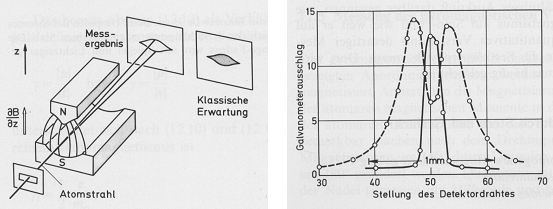
\includegraphics[width=\textwidth]{fig/3-SternGerlachExperiment.png}
	\caption{Aufbau des Stern-Gerlach Experiments}
\end{figure}

Im Experiment wurde ein Silberstrahl durch ein sehr inhomogenes Magnetfeld
auf eine Fotoplatte gestrahlt. Die neutralen Silberatome besitzen ein
magnetisches Moment, das sich am Feld ausrichtet. Klassisch müsste jede
Ausrichtung des magnetischen Moments möglich sein und daher ist eine
kontinuierliche Verteilung im Magnetfeld zu erwarten.

Die quantenmechanische Betrachtung besagt, dass die Atome abhängig von ihrem 
$\mu_z$-Zustand diskrete Winkel einstellen. Diejenigen mit $\mu_z = 0$ werden
das Magnetfeld gerade durchqueren, andere werden sich zu den Bereichen
mit dichteren bzw. dünneren Magnetfeldlininen verschieben. Geht man davon aus,
dass alle Atome sich im gleichen $l$-Zustand befinden, müssten nach unserer
bisherigen Überlegung auf der Platte $2l+1$, d.h. eine ungerade Zahl
3,5,7,\ldots an Linien zu sehen sein. Man sah jedoch genau 2. Ursache hierfür
ist der Spin der Elektronen im Silber $s=\frac{1}{2}\Rightarrow 2s+1 = 2$.

Zu diesem Zeitpunkt wusste man jedoch noch nichts über den Spin und dass die
Elektronen im Silber im Grundzustand Spin $\frac{1}{2}$ und Drehimpuls Null
haben. Für einen Nachweis der Aufspaltung reichte der Befund jedoch aus. 1927,
6 Jahre später, haben Phipps und Taylor die Aufspaltung in zwei Linien auch
beim Wasserstoff nachgewiesen.

% TODO: Weglassen oder Herr Pfau fragen 
% Im Silberatom tragen die Elektronen in den ``geschlossenen Schalen'' nichts
% zum Spin bei, da dieser sich gerade wegmittelt
% ($\uparrow\downarrow\uparrow\downarrow$). Dennoch stehen mehrere
% ``Valenzelektronen'' zur Verfügung. Die Frage ist nun, wie das magentische
% Moment aufgrund des Bahndrehimpulses und das aufgrund des Spins zu einem
% Gesamtdrehimpuls koppeln.

Das Experiment zeigt, dass es neben dem magnetischen Moment hervorgerufen durch
den Bahndrehimpuls $l$ auch eines aufgrund des Spins $s$ gibt,
\begin{align*}
\op{\mu}_s = g_s \mu_B \frac{\op{s}}{\hbar}.
\end{align*}
Der Elektronenspin ist auch makroskopisch messbar, was bereits 1915 im
Einstein-de-Haas-Experiment\footnote{Wander Johannes de Haas (* 2. März 1878 in
Lisse nahe Leiden; † 26. April 1960 in Bilthoven) war ein niederländischer
Physiker und Mathematiker.} durchgeführt wurde. Dabei beobachtet man einen
einen Eisenstab im homogenen Magnetfeld. Dieses führt dazu, dass sich die
Elektronenspins in eine Richtung ausrichten. Kehrt man nun das Magnetfeld um,
drehen sich auch die magnetischen Momente des Spins, was zu einem Drehmoment
führt. Dieses Drehmoment kann man messen und damit $g_s$ berechnen.
\begin{align*}
\Rightarrow g_s \approx 2.
\end{align*}
Der Spin erzeugt also ein dopplet so großes magnetisches Moment, wie eine
klassisch mit $\frac{1}{2}\hbar$ rotierende geladene Kugel.  Das magnetische
Moment aufgrund des Spins ``funktioniert'' also anders als das aufgrund des
klassischen Bahndrehimpulses. Es ist ein rein quantenmechanischer Effekt ohne
klassischen Grenzfall.

Um den $g$-Faktor des Spins zu erklären, müssen wir relativistische Effekte
berücksichtigen. Die Schrödingergleichung ist eine nichtrelativistische
Gleichung. Dirac\footnote{Paul Adrien Maurice Dirac, OM (* 8. August 1902 in
Bristol; † 20. Oktober 1984 in Tallahassee) war ein britischer Physiker,
Nobelpreisträger für Physik des Jahres 1933 und Mitbegründer der
Quantenphysik.} erweiterte die Schrödingergleichung auf die spezielle
Relativitätstheorie, indem er forderte, dass sie die relativistische
Energie-Impuls-Beziehung erfüllen muss und nur eine 1. Ableitung nach der Zeit
enthalten darf.

Er stellte fest, dass nur eine Wellenfunktion, die von mindestens 4 Parametern
abhängt, diese Forderungen erfüllen kann. Das erste Parameterpaar stellt dabei
das Teilchen mit Spin Up und Down dar und das zweite Parameterpaar das
Antiteilchen mit Spin Up und Down.

Dirac errechnete mit dieser Theorie, dass $g_s=2$ exakt. Der Nobelpreisträger
Dehmelt\footnote{Hans Georg Dehmelt (* 9. September 1922 in Görlitz) ist ein
deutsch-US-amerikanischer Physiker und Nobelpreisträger für Physik des Jahres
1989.} bestimmte jedoch 1987 die Größe experimentell mit sehr hoher Präzession auf,
\begin{align*}
g_s = 2.002319304386.
\end{align*}
Feynman\footnote{Richard Phillips Feynman (* 11. Mai 1918 in New
York; † 15. Februar 1988 in Los Angeles) war ein US-amerikanischer Physiker
und Nobelpreisträger für Physik des Jahres 1965.} erweiterte die Theorie von
Dirac durch die Korrekturterme,
\begin{align*}
g_s = 2.00 \left(1 + \frac{\alpha}{2\pi} + \ldots \right),\qquad \alpha \text{
Feinstrukturkonstante}
\end{align*}
und war damit in der Lage auch die Nachkommastellen korrekt vorherzusagen. Der
Unterschied zwischen theoretischem und empirisch ermittelten Wert beträgt
heute $\frac{\Delta g}{g} = 10^{-11}$.

Dies ist auch ein Anhaltspunkt dafür, wie ``gut'' die Quantenmechanik ist. Jede
Theorie, die die Quantenmechanik wiederlegen bzw. ersetzen will, müsste
mindestens die selbe Präzession erreichen.

\subsubsection{Addition von Drehimpulsen}

Wir wollen nun den Fall untersuchen, wenn sowohl Spin als auch
Bahndrehimpuls vorhanden sind. Klassisch addieren sich Bahndrehimpuls $\vec{l}$
und Spin $\vec{s}$ vektroriell zum Gesamtdrehimpuls $\vec{j}$,
\begin{align*}
\vec{j} = \vec{l} + \vec{s}.
\end{align*}

In der Quantenmechanik sind $\op{s}$ und $\op{l}$ unscharf, z.B. sind nur
Betrag und die $z$-Komponente bekannt und daher $x$- und $y$-Komponente
unscharf. Diese Unschärfe überträgt sich auch auf $\op{j}$.

\begin{figure}[!htbp]
\centering
\begin{pspicture}(0,-1.534)(3,1.534)
\psellipse(0.99,0.76)(0.99,0.41)
\psline(0.98,-1.25)(0.0,0.73)
\psline(2.16,0.09)(2.76,0.39)
\psline{->}(0.98,-1.53)(0.98,1.53)
\psline[linestyle=dotted,dotsep=0.06cm](1.96,0.73)(0.98,0.73)
\psline(0.98,-1.23)(1.34,0.49)

%\rput{-23.744934}(0.40731186,0.4171894){\psellipse(1.1958715,-0.76012886)(0.42806548,0.14858808)}
%\rput{-26.793932}(0.060014352,0.82076675){\psellipse(1.753021,0.28439686)(0.4606442,0.1815386)}

\rput{-23.744934}(-0.032369815,1.0057698){\psellipse(2.3758714,0.5798712)(0.42806548,0.14858808)}
\rput{-26.793932}(0.06001435,0.82076675){\psellipse(1.753021,0.28439686)(0.4606442,0.1815386)}

\psline[linecolor=darkblue]{->}(0.98,-1.25)(1.98,0.73)
\psline[linecolor=purple]{->}(0.98,-1.25)(2.18,0.09)
\psline[linecolor=yellow]{->}(2.16,0.09)(1.98,0.73)
%\psline[linecolor=yellow]{->}(0.98,-1.25)(0.8,-0.61)

\rput(2.05,-0.385){\color{purple}$\op{l}$}

\rput(2.27,0.3){\color{yellow}$\op{s}$}

\rput(2.14,1.1){\color{darkblue}$\op{j}$}

\rput(0.8,0.915){\color{gdarkgray}$\op{j}_z$}

%\rput(0.7,-0.985){\color{yellow}$\op{s}$}
\end{pspicture}
\begin{pspicture}(0,-1.5511667)(2.7977192,1.5511667)
\psellipse(0.99,-0.54705554)(0.99,0.41)
\psline(0.98,-1.26)(0,-0.58)
\psline(2.16,0.06119258)(2.725889,-0.20294444)
\psline{->}(0.9858889,-1.5370556)(0.9858889,1.5370556)
\psline[linestyle=dotted,dotsep=0.06cm](1.96,-0.59705555)(0.98,-0.59705555)
\psline(0.98,-1.2370555)(1.34,0.48294446)
\rput{24.358875}(0.042940438,-1.0163105){\psellipse(2.3758714,-0.4086787)(0.42806548,0.14858796)}
\rput{-26.793932}(0.06319487,0.82000923){\psellipse(1.753021,0.2773413)(0.4606442,0.1815386)}
\psline[linecolor=darkblue]{->}(0.98,-1.2570555)(1.9858888,-0.58294445)
\psline[linecolor=yellow]{->}(2.16,0.06119258)(1.98,-0.5788074)
\psline[linecolor=purple]{->}(0.98,-1.2570555)(2.18,0.082944445)

\rput(2.215889,-0.175){\color{yellow}$\op{s}$}
\rput(1.4458889,-1.1779444){\color{darkblue}$\op{j}$}
\rput(2.275889,0.23){\color{purple}$\op{l}$}
\rput(0.82,-0.51794446){\color{gdarkgray}$\op{j}_z$}
\end{pspicture} 

\caption{Addition von $\op{s}$ und $\op{l}$ zu $\op{j}$. Maximale Einstellung
(links) und minimale Einstellung (rechts).}
\end{figure}

Die Eigenwertgleichungen des Gesamtdrehimpulses $\op{j}$ ergeben sich analog
zu den des Drehimpulses $\op{l}$ und des Spins $\op{s}$,
\begin{align*}
&\op{l}^2\ket{l,m_l} = l(l+1)\hbar^2\ket{l,m_l},\\
&\op{s}^2\ket{s,m_s} = s(s+1)\hbar^2\ket{s,m_s},\\
\Rightarrow\;&\op{j}^2\ket{j,m_j} = j(j+1)\hbar^2\ket{j,m_j},\\
&\op{l}_z\ket{l,m_l} = m_l\hbar\ket{l,m_l},\\
&\op{s}_z\ket{s,m_s} = m_s\hbar\ket{s,m_s},\\
\Rightarrow\;&\op{j}_z\ket{j,m_j} = m_j\hbar\ket{j,m_j}.
\end{align*}
Über die Eigenwerte wissen wir,
\begin{align*}
&l\le n-1,\quad
m_l = -l,\ldots,l,\quad
m_s = -s,\ldots,s.
\end{align*}
Wie verhält es sich nun mit den Eigenwerten des Gesamtdrehimpulses?
\begin{align*}
&\op{j}_z = \op{l}_z + \op{s}_z,\qquad
\Rightarrow  m_j = m_l + m_s,
\end{align*}
Wir können also Maximal- und Minimalwerte von $m_j$ angeben und damit auch den
Wertebereich von $j$. Für $l>s$ gilt,
\begin{align*}
& m_j^{\small\text{max}} =
m_l^{\small\text{max}} + m_s^{\small\text{max}} = l+s = j^{\small\text{max}},\\
& m_j^{\small\text{min}} =
m_l^{\small\text{min}} + m_s^{\small\text{min}} = l-s = j^{\small\text{min}},\\
\Rightarrow & j = l-s,l-s+1,\ldots,l+s. 
\end{align*}
Für ein einzelnes Elektron ist $s=\frac{1}{2}$, d.h. es gibt zu gegebenem
$l$ jeweils nur zwei mögliche Gesamtdrehimpulse $j$ (außer für $l=0$). Für $m_j$
gibt es dafür $2j+1$ Einstellmöglichkeiten.
\begin{figure}
\centering
\begin{pspicture}(-0.1,-1.4)(3.6,1.8)
\psline{->}(1.06,-1.31)(1.06,1.31)
\psarc(1.06,-0.13){1.06}{270.0}{90.0}
\psline[linecolor=darkblue]{->}(1.06,-0.11)(1.84,0.5841111)
\psline[linecolor=darkblue]{->}(1.06,-0.09)(1.86,-0.8158889)
\psline[linecolor=darkblue]{->}(1.06,-0.11)(2.08,0.16411111)
\psline[linecolor=darkblue]{->}(1.06,-0.09588889)(2.1,-0.3358889)

\psline[linestyle=dotted,dotsep=0.06cm](1.06,0.15)(2.08,0.16411111)
\psline[linestyle=dotted,dotsep=0.06cm](1.06,-0.33)(2.1,-0.31588888)
\psline[linestyle=dotted,dotsep=0.06cm](1.06,0.59)(1.84,0.59)
\psline[linestyle=dotted,dotsep=0.06cm](1.86,-0.81)(1.06,-0.81)

\rput(0.83,1.4){\color{gdarkgray}$\op{j}_z$}
\rput(2.76,1.4){\color{gdarkgray}$m_j$}

\rput[r](3,0.6){\color{gdarkgray}$3/2$}
\rput[r](3,0.15){\color{gdarkgray}$1/2$}
\rput[r](3,-0.35){\color{gdarkgray}$-1/2$}
\rput[r](3,-0.8){\color{gdarkgray}$-3/2$}

\rput[r](0.9,0.6){\color{gdarkgray}$3/2\hbar$}
\rput[r](0.9,0.15){\color{gdarkgray}$1/2\hbar$}
\rput[r](0.9,-0.35){\color{gdarkgray}$-1/2\hbar$}
\rput[r](0.9,-0.8){\color{gdarkgray}$-3/2\hbar$}
\end{pspicture} 
\caption{Einstellmöglichkeiten für $\op{j}_z$ für $j=\frac{3}{2}\hbar$}
\end{figure}

\begin{bspn}
$l=2$, $s=\frac{1}{2}$, dann ist $j=\frac{3}{2}$ oder $\frac{5}{2}$.\bsphere
\end{bspn}

\begin{figure}[!htbp]
\begin{tabular}{r|c|c|c|c}
 & $s$ & $p$ & $d$ & $f$\\
$l$ & $0$ & $1$ & $2$ & $3$\\\hline
$j$ & $\frac{1}{2}$ & $\frac{1}{2}$, $\frac{3}{2}$ & $\frac{3}{2}$,
$\frac{5}{2}$ & $\frac{5}{2}$, $\frac{7}{2}$\\\hline
Notation & $S_{1/2}$ & $P_{3/2}$, $P_{3/2}$ & $D_{3/2}$, $D_{5/2}$ & $F_{5/2}$,
$F_{7/2}$
\end{tabular}
\caption{Mögliche Gesamtdrehimpulse für ein Einelektronen-Atom.}
\end{figure}

\newpage
\subsection{Atome im Magnetfeld - Zeeman Effekt}

Um zu verstehen, wie sich Atome im Magnetfeld verhalten, müssen wir untersuchen,
wie das magnetische Moment des Drehimpulses $\op{\mu}_l$ und das des
Spins $\op{\mu}_s$ zu einem Gesamtmoment $\op{\mu}_j$ koppeln.

Während $\op{\mu}_s\parallel \op{s}$ und $\op{\mu}_l\parallel \op{l}$, gilt
aufgrund der verschiedenen $g$-Faktoren für $s$ und $l$ nun
$\op{\mu}_j\nparallel \op{j}$.

Des Weiteren sind $\op{l}$ und $\op{s}$ durch die magnetische
Wechselwirkung aneinander gekoppelt. Dabei wechselwirken die 
magnetischen Momente (Dipol/Dipol-Wechselwirkung) und resultieren in konstanten
Energiewerten. Z.B. wird die Wechselwirkungsenergie im tiefsten Zustand
konstant minimal gehalten.

Unser Ziel ist es nun, $\op{\mu}_j$ durch Größen auszudrücken, die wir
gleichzeitig messen können, das sind
\begin{align*}
\op{j}_z, \op{j}^2, \op{l}^2, \op{s}^2.
\end{align*}

\subsubsection{Klassische Betrachtung}

Zeeman beobachtete (1896) eine Aufspaltung der Spektrallininen im Magnetfeld,
lange bevor man überhaupt ein Verständinis über das Zustandekommen der
Spektrallinien hatte.

Das klassische Modell geht zurück auf Lorentz. Wir betrachten ein Elektron auf
einer festen Kreisbahn mit Radius $r$, Zentrifugal- und Coulombkraft
kompensieren sich gerade.

Im Magnetfeld wirkt aufgrund der Bewegung eine zusätzliche Kraft, die
Lorentzkraft,
\begin{align*}
&F_L = \frac{1}{c}e\left(\vec{v}\times \vec{B}\right) = \frac{1}{c}e\omega' r
B,\\
\Rightarrow & m\omega^2 r = m\omega'^2r + \frac{1}{c} e \omega' rB,\\
\Leftrightarrow & \frac{m\left(\omega^2 - \omega'^2 \right)}{\omega'} =
\frac{1}{c}eB.
\end{align*}
Entwickle in $\omega$ mit $\Delta \omega = \omega - \omega'$
\begin{align*}
&\frac{\omega^2 - \omega'^2}{\omega'} = 
\frac{\left(\Delta\omega + \omega'\right)^2 - \omega'^2}{\omega'}
= \frac{\Delta \omega^2 + 2\omega'\Delta\omega + \omega'^2 -
\omega'^2}{\omega'}
\approx 2\Delta \omega\\
\Rightarrow &\Delta \omega = \pm \frac{eB}{2mc} = \pm
\omega_{\text{Larmor}}
\end{align*}
Je nach Umlaufsinn wird daher das Elektron schneller bzw. langsamer.

\begin{figure}[!htbp]
\centering
\begin{pspicture}(0,-1.41)(7.09,1.41)
\psline[linestyle=dotted,dotsep=0.06cm](1.4,-0.09)(1.4,1.11)
\psline[linecolor=darkblue](0.2,-0.09)(0.2,1.11)
\psline[linecolor=purple](2.58,-0.09)(2.58,1.11)
\psline{->}(0.0,-0.09)(3.02,-0.09)

\rput(0.25,1.255){\color{gdarkgray}$\sigma^-$}
\rput(2.65,1.255){\color{gdarkgray}$\sigma^+$}
\rput(2.85,-0.225){\color{gdarkgray}$\omega$}
\rput(1.9,-0.345){\color{gdarkgray}$\omega_L$}
\psline(1.4,-0.21)(1.4,-0.09)
\psline(2.58,-0.09)(2.58,-0.21)

\rput(1.41,-0.785){\color{gdarkgray}2 Linien}

\psline[linecolor=yellow](5.46,-0.09)(5.46,1.11)
\psline[linecolor=darkblue](4.26,-0.09)(4.26,1.11)
\psline[linecolor=purple](6.64,-0.09)(6.64,1.11)
\psline{->}(4.06,-0.09)(7.08,-0.09)

\psline{<->}(6.4,0.91)(6.9,0.91)
\psline{<->}(5.38,0.43)(5.38,1.01)
\psline{<->}(4.02,0.91)(4.52,0.91)

\rput(4.31,1.255){\color{gdarkgray}$\sigma^-$}
\rput(6.71,1.255){\color{gdarkgray}$\sigma^+$}
\rput(6.91,-0.225){\color{gdarkgray}$\omega$}
\rput(5.5,-0.305){\color{gdarkgray}$\omega_0$}
\rput(5.47,1.275){\color{gdarkgray}$\pi$}

\rput(5.47,-0.785){\color{gdarkgray}3 Linien}

\rput(1.4,-1.185){\color{gdarkgray}z-Richtung}
\rput(5.48,-1.185){\color{gdarkgray}x,y-Ebene}
\end{pspicture} 
\caption{Spektrum des Zeeman-Effekts (schematisch).}
\end{figure}

Klassisch ist das Elektron als ``rotierende Antenne'' zu verstehen.
In $z$-Richtung beobachtet man links- und rechts zirkular polarisiertes Licht,
sogenanntes $\sigma^-$ bzw. $\sigma^+$-Licht.
In der $x,y$-Ebene beobachtet man neben dem in $z$-Richtung zirkular
polarisiertem $\sigma^-$ und $\sigma^+$ Licht, auch noch
linear polarisierts $\pi$-Licht.
Dies nennt man den \emph{normalen Zeeman-Effekt}.

\sfigure[H][0.6]%
	{3-AufspaltungNormalerZeemanEffekt.pdf}
	{\HertelSchulz, S. 287}
	{Aufspaltung bei normalen Zeeman-Effekt.}

\subsubsection{Quantenmechanische Betrachtung}

Das Elektron hat einen Bahndrehimpuls $\op{l}$ und einen Spin $\op{s}$,
der Gesamtdrehimpuls ist $\op{j}$. Wie verhält es sich nun mit dem
gesamtmagnetischen Moment?
\begin{align*}
\op{\mu}_j = \op{\mu}_s + \op{\mu}_l
= g_s \mu_B \frac{\op{s}}{\hbar} + g_l \mu_B \frac{\op{l}}{\hbar}
= \frac{\mu_B}{\hbar} \left(2\op{s} + \op{l}\right)
= \frac{\mu_B}{\hbar} \left(\op{j} + \op{s}\right)
 \nparallel \op{j}.
\end{align*}

\begin{figure}[!htbp]
\centering
\begin{pspicture}(0,-2.152)(2.38,2.18)
\psline[linecolor=darkblue]{->}(0.98,-0.2)(1.98,1.78)
\psline[linecolor=purple]{->}(0.98,-0.2)(2.18,1.14)
\psline[linecolor=yellow]{->}(2.16,1.14)(1.98,1.78)

\psline[linecolor=purple]{->}(0.98,-0.2)(0.42,-0.86)
\psline[linecolor=yellow]{->}(0.42,-0.86)(0.6,-1.5)
\psline[linecolor=darkblue]{->}(0.98,-0.2)(0.6,-1.46)

\psline[linestyle=dotted,dotsep=0.06cm]{<-}(0.02,-2.14)(1.02,-0.16)

\rput(2.05,0.665){\color{gdarkgray}$\vec{l}$}

\rput(2.27,1.505){\color{gdarkgray}$\vec{s}$}

\rput(1.6,1.65){\color{darkblue}$\vec{j}$}

\rput(0.47,-0.355){\color{gdarkgray}$\vec{\mu}_l$}

\rput(0.19,-1.135){\color{gdarkgray}$\vec{\mu}_s$}

\rput(1.08,-0.915){\color{darkblue}$\vec{\mu}_j$}
\end{pspicture}
\caption{Addition von $\vec{\mu}_s$ und $\vec{\mu}_l$ im Vergleich zu $\vec{s}$
und $\vec{l}$.}
\end{figure}

Wir wollen nun die Wechselwirkungsenergie des gesamtmagnetischen Moments mit
einem äußeren Magnetfeld berechnen. Dabei gehen wir zunächst davon aus, dass
dieses Feld ``schwach'' ist und die Orientierung von $\mu_s$ und $\mu_l$ nicht
verändert wird.
\begin{align*}
V_B = -\op{\mu}_j \op{B}.
\end{align*}
Um in einer ``guten Basis'' zu rechnen, projezieren wir $\op{\mu}$ auf
$\op{j}$ und $\vec{B}$ auf $\op{j}$,
\begin{align*}
V_B
=
\left(-\op{\mu}_j\frac{\op{j}}{\abs{\op{j}}}\right)\left(\frac{\op{j}}{\abs{\op{j}}}\op{B}\right)
=
\frac{\mu_B}{\hbar}\frac{\left(\op{s}+\op{j}\right)\op{j}\left(\op{j}\op{B}\right)}{\op{j}^2}
= \frac{\mu_B}{\hbar} B \op{j}_z \left(\frac{\op{j}^2 +
\op{s}\op{j}}{\op{j}^2}\right).
\end{align*} 
Wir wollen diesen Ausdruck nun auf Größen reduzieren, die wir gleichzeitig
messen können. Betrachte dazu,
\begin{align*}
\op{l}^2 = \left(\op{s}+\op{j}\right)^2 = \op{j}^2 + 2\op{s}\op{j} +
\op{s}^2.
\end{align*}
Einsetzen ergibt,
\begin{align*}
V_B = \frac{\mu_B}{\hbar} B \op{j}_z \left(\frac{\op{j}^2 - \frac{\op{j}^2 -
\op{l}^2 + \op{s}^2}{2}}{\op{j}^2} \right)
\end{align*}
Wir haben damit $V_B$ durch gleichzeitig messbare Größen ausgedrückt. Ersetzen
der Operatoren durch Eigenwerte, ergibt sich
\begin{align*}
\Delta E = \mu_B B m_j \underbrace{\left[ \frac{j(j+1) + \frac{1}{2}\left(j(j+1)
+ s(s+1) - l(l+1) \right)}{j(j+1)}\right]}_{:= g_j}.
\end{align*}
$g_j$ nennt man den \emph{Landé'schen
$g$-Faktor}, $g_j\in[1,2]$.
Die Energieaufspaltung aufgrund des Zeeman-Effekts findet also in
$2j+1$ äquidistante Niveaus statt.

\begin{bemn}[Bemerkungen.]
\begin{enumerate}[label=\arabic{*}.)]
  \item $s=0\Rightarrow j=l, g_j = 1 = g_l$,\\
$l=0\Rightarrow j=s, g_j = 2 = g_s$.
\item 
Übergänge zwischen den Niveaus können nur für $\Delta m_j = 0,\pm 1$
stattfinden. 
\item
Der \emph{normale Zeeman-Effekt} tritt auf, wenn der $g$-Faktor im angeregten
und im Grundzustand gleich ist. D.h. $s=0$, denn ein Übergang erfordert
$\Delta l = \pm 1$, dies ist nur bei
Mehrelektronen-Atomen möglich. Die Energieniveaus spalten sich dabei in eine
ungerade Anzahl $2l+1$ auf.

Der \emph{annomale Zeeman-Effekt} tritt in allen anderen Fällen auf. Die
Anzahl der Energieniveaus $2j+1$ kann hier auch gerade sein, wenn $j$
halbzahlig ist

Der normale Zeeman Effekt tritt also nur auf, wenn der Spin keine Rolle
spielt. Der annomale Zeeman-Effekt ist somit häufiger anzutreffen.\maphere
\end{enumerate}
\end{bemn}
 
\begin{bemn}[Ausblick.]
Im Abschnitt über Kernphysik haben wir gesehen, dass auch Protonen und
Neutronen einen Spin besitzen. Dieser kann ebenfalls mit den magnetischen
Momenten der Elektronen wechselwirken.

\begin{table}[h]
\begin{tabular}{l|c|l}
& \text{Spin} & \text{Landé-Faktor}\\\hline
Proton & $ \frac{1}{2}$ & $g_p = 5.586\ldots$\\
Neutron & $\frac{1}{2}$ & $g_n = -3.826\ldots$
\end{tabular}
\end{table}

Diese Wechselwirkung werden wir im Rahmen der Hyperfeinstruktur genauer
untersuchen.\maphere
\end{bemn}

\subsection{Feinstruktur}

Im Experiment sehen wir für gleiches $l$ aber unterschiedliches $j$ eine
weitere Aufspaltung der Energieniveaus. Sie heißt
\emph{Feinstrukturaufspaltung} und fasst mehrere Phänomenen zusammen. Um diese
zu erklären, müssen wir unser Modell weiter verfeinern. Dazu werden wir
zunächst die Kopplung des Spins $s$ und des Bahndrehimpulses $l$ untersuchen.
Anschließend werden wir - wie bereits im Bohr-Sommerfeld-Modell -
relativistische Korrekturen einführen, denn magnetische Phänomene sind
relativistische Wechselwirkungen 1. Ordnung.

\subsubsection{Spin-Bahn-Wechselwirkung}

Die Wechselwirkung des magnetischen Moments des Spins mit dem Magnetfeld
aufgrund der Bahnbewegung des Elektrons ruft eine Aufspaltung der Energieniveaus
hervor
\begin{align*}
\Delta E_{ls} = -\vec{\mu}_s\cdot \vec{B}_l,
\end{align*} 
wobei $\vec{\mu}_s$ das magnetische Moment des Spins im Ruhesystem des
Elektrons und $\vec{B}_l$ das Magnetfeld aufgrund des Bahndrehimpules $\vec{l}$
am Ort des Elektrons beschreibt.

\begin{figure}[!htbp]
\centering
\begin{pspicture}(0,-0.91411114)(1.94,0.91411114)

\psellipse[linestyle=dotted,dotsep=0.06cm](0.78,0.02)(0.78,0.32)
\psline{->}(1.42,0.2)(1.72,-0.02)
\psline[linecolor=darkblue]{->}(0.78,0.02)(0.78,0.9)
\psline{->}(0.78,0.02)(1.38,0.18)
\psdots[linecolor=yellow](1.42,0.2)

\rput(1.85,0.06){\color{gdarkgray}$\vec{v}$}
\rput(1.1,-0.05){\color{gdarkgray}$r$}
\rput(1.5,0.45){\color{gdarkgray}$e^-$}
\rput(0.58,0.785){\color{gdarkgray}$\vec{B}$}
\end{pspicture} 
 
\caption{Bewegung des Elektrons.}
\end{figure}

Das Ruhesystem des Elektrons ist jedoch ein beschleunigtes Bezugssystem
(Kreisbewegung), d.h. \textit{kein} Inertialsytem. Berechnen wir zunächst das
Magnetfeld mit dem Biot-Savart'schen Gesetz in diesem Bezugssystem,
\begin{align*}
\vec{B}_l = \frac{I}{c} \int\limits_0^{2\pi} \frac{\dvecs \times \vec{r}}{r^3}
= -\frac{eZ}{c}\frac{\vec{v}\times \vec{r}}{r^3}
= \frac{eZ}{mcr^3}\vec{l},
\end{align*}
müssen wir das Ergebnis ins Laborsystem zurücktransformieren. Die etwas
längliche Rechnung sei als Übungsaufgabe überlassen. Es ergibt sich,
\begin{align*}
\vec{B}_l = \frac{1}{2}\frac{Ze}{mcr^3}\vec{l}.
\end{align*}
Der Faktor $\frac{1}{2}$ heißt Thomas-Faktor und entsteht bei Transformation
von Nichtinertialsystemen. Übertragen wir dieses Ergebnis auf Operatoren
mit $\op{\mu}_s = -2\mu_B \frac{\op{s}}{\hbar}$ für $g_s = 2$
erhalten wir,
\begin{align*}
\Delta E_{ls} = -\op{\mu}_s \op{B}_l = 2\frac{e\hbar}{2mc}\frac{Ze}{2mcr^3}
\frac{\op{l}\op{s}}{\hbar} = \underbrace{\frac{Ze^2}{2m^2
c^2r^3}}_{\rho(r)}\op{l}\op{s}.
\end{align*}
Diesen Ausdruck kann man als Dipol/Dipol-Wechselwirkung identifizieren. Mit dem
Erwartungswert des H-Atoms von $\frac{1}{r^3}$ kann $\Delta E_{ls}$ berechnet
werden,
\begin{align*}
\Delta E_{ls} \approx 10^{-4}\mathrm{eV} \entspr 24.2 \mathrm{GHz}\quad
\Rightarrow\quad \frac{\Delta E_{ls}}{E}\approx 10^{-5}\mathrm{eV}.
\end{align*}
Der Wert ist klein im Vergleich zur Bindungsenergie aber relativ groß im
Frequenzspektrum, daher ist er auch schon so früh entdeckt worden.

Die Größe des Magnetfeldes das vom Bahndrehimpuls erzeugt wird,
\begin{align*}
B_l = \frac{\Delta E_{ls}}{\mu_B} =
\frac{10^{-4}\mathrm{eV}}{\mu_B} \approx 1T.
\end{align*}
Die Forderung, dass das äußere Magnetfeld ``schwach'' sein soll, bezieht sich
auf diese Größe. Erst wenn äußere Magnetfelder der Größenordnung 
$1\mathrm{T}$ anliegen, wird die Kopplung von $s$ und $l$ beeinflusst.

Betrachten wir nun die Änderung des Hamilton-Operators,
\begin{align*}
\op{H}_{\text{FS}} = \rho(r)\; \op{l}\op{s},
\end{align*}
und verwenden $\op{l}\op{s} = \frac{1}{2}\left(\op{j}^2 - \op{l}^2 -
\op{s}^2\right)$, ergibt sich
\begin{align*}
\lin{\Delta E_{ls}} = \lin{\op{H}_{\text{FS}}} = \lin{\rho(r)\op{l}\op{s}} = 
\lin{\rho(r)}\frac{\hbar^2}{2}\left[ j(j+1) - l(l+1)-s(s+1) \right],
\end{align*}
wobei $\lin{\rho(r)} = \frac{a}{\hbar^2}$. $a$ heißt
\emph{Spin-Bahn-Kopplungskonstante}. Für das H-Atom ist
\begin{align*}
\lin{\Delta E_{ls}} = a\cdot
\begin{cases}
\frac{l}{2},& \text{für }j=l+\frac{1}{2},\\
-\frac{l+1}{2},& \text{für }j=l-\frac{1}{2}.
\end{cases}
\end{align*}
\begin{figure}
\centering
\begin{pspicture}(0,-1.8)(9,1.8)
\psline(0.0,0.24)(1.0,0.24)
\psline[linecolor=darkblue,linestyle=dotted,dotsep=0.06cm](1.02,0.24)(1.82,0.84)
\psline[linecolor=purple,linestyle=dotted,dotsep=0.06cm](1.02,0.24)(1.82,-1.36)
\psline[linecolor=darkblue](1.82,0.86)(3.42,0.86)
\psline[linecolor=purple](1.82,-1.36)(3.42,-1.36)
\psline[linestyle=dotted,dotsep=0.06cm](1.06,0.24)(3.42,0.24)
\psline{<->}(2.0,0.78)(2.0,0.32)
\psline{<->}(2.0,0.16)(2.0,-1.28)

\rput(2.38,0.565){\color{gdarkgray}$a/2$}
\rput(2.28,-0.515){\color{gdarkgray}$-a$}
\rput(3.02,1.085){\color{gdarkgray}$2P_{3/2}$}
\rput(3.02,-1.575){\color{gdarkgray}$2P_{1/2}$}
\rput(4.33,1.625){\color{gdarkgray}Entartung}
\rput(4.3,1.085){\color{gdarkgray}4x}
\rput(4.3,-1.575){\color{gdarkgray}2x}
\rput[l](5,1.085){\color{gdarkgray}$m_j=-3/2,-1/2,1/2,3/2$}
\rput[l](5,-1.575){\color{gdarkgray}$m_j=-1/2,1/2$}
\end{pspicture}
\caption{Aufspaltung durch
Spin-Bahn-Wechselwirkung.}
\end{figure}

Die Lorentzkraft wirkt $\bot$ zur Bewegungsrichtung und verrichtet daher keine
Arbeit. Es kann somit nicht zur Verschiebung der Energie kommen. Wir sehen
dies auch bei der Aufspaltung, denn ${}^2 P_{3/2}$ ist 4-fach entartet, während
${}^2P_{1/2}$ lediglich 2-fach entartet ist. Der Linienschwerpunkt bleibt daher
erhalten. Für $l=0$ haben wir keine Aufspaltung.

Betrachten wir die Größe $a$ genauer,
\begin{align*}
a&:= \hbar^2 \lin{\rho(r)} = \hbar^2 \int R_{nl}^* \rho(r) R_{nl} r^2\dr
\ldots\\ &= \frac{mc^2}{2}(Z\alpha)^4 \frac{1}{n^3(l(l+\frac{1}{2})(l+1))},
\end{align*}
so ergibt sich als Energieskala die Ruheenergie $\frac{mc^2}{2}$.

Wenn wir die Spin-Bahn-Wechselwirkung in $\alpha$ entwickeln, hat diese die
Ordnung $\alpha^4$. Um die Wirkung vollständig zu beschreiben, müssen wir daher nach
anderen Effekten suchen, die die selbe Ordnung haben.

\subsubsection{Relativistische Massenzunahme}

Betrachte den relativistischen Ausdruck für die Energie des Elektrons,
\begin{align*}
E = c\sqrt{\vec{p}^2 + m^2 c^2}.
\end{align*}
und entwickle in $\vec{p}$, so ergibt sich
\begin{align*}
E = mc^2 + \frac{\vec{p}^2}{2m} - \frac{\vec{p}^4}{8m^3 c^2} + \ldots.
\end{align*}
Verglichen mit der Energie $\frac{\vec{p}^2}{2m}$ gilt für den ersten
relativistischen Korrekturterm
\begin{align*}
\frac{\vec{p}^4/8m^3 c^2}{\vec{p}^2/2m} = 4m^2\frac{\vec{p}^2}{c^2}
\sim
\left(\frac{v}{c}\right)^2 \approx \alpha^2 \sim 5\cdot 10^{-5}.
\end{align*}
Die Korrektur der relativistischen Massenzunahme hat daher die Ordnung
$\alpha^4$ und somit dieselbe Ordnung in $\alpha$ wie die
Spin-Bahn-Wechselwirkung. Sie erzeugt daher vergleichbar starke Effekte.

Für eine exakte Rechnung müssten wir nun zur relativistischen
Schrödingergleichung (Dirac) übergehen. Wir wollen uns jedoch mit Korrekturen
bis zur 4. Ordnung begnügen. Wenden wir die Störungstheorie auf die
H-Wellenfunktion an, ergibt sich,
\begin{align*}
\lin{\Delta E_{\text{rel}}} &= -\frac{\hbar^2}{8m^3c^4}\int_{\R^3} \Psi_{nlm}^*
\nabla^4 \Psi_{nlm} \dV \\
 &=
-\frac{mc^2}{2}\left(Z\alpha\right)^4\left(\frac{1}{n^3\left(l
+ \frac{1}{2}\right)} - \frac{3}{4n^4}\right).
\end{align*}

\subsubsection{Feinstrukturaufspaltung.}

Wir wollen nun die Abweichung aufgrund der Spin-Bahn-Wechselwirkung und der
relativistische Massenzunahme in der Feinstrukturaufspaltung zusammenfassen,
\begin{align*}
\Delta E_{\text{FS}} = \Delta E_{ls} + \Delta E_{\text{rel}}.
\end{align*}
Für das H-Atom mit $j=l\pm\frac{1}{2}$ ergibt sich somit,
\begin{align*}
\lin{\Delta E_\text{FS}} = -\frac{1}{2}mc^2\left(Z\alpha\right)^4
\frac{1}{n^3}\left( \frac{1}{j+\frac{1}{2}} - \frac{3}{4n},
\right).
\end{align*}
$\Delta E_{\text{FS}}$ ist also unabhängig von $l$, d.h. Zustände mit gleichem
$j$ aber unterschiedlichem $l$ und $s$ sind weiter entartet.

\begin{figure}[!htbp]
\centering
\begin{pspicture}(-0.4,-1.62)(8.36,1.62)
\psline[linecolor=darkblue](0.0,0.64)(0.82,0.64)
\psline[linecolor=purple,linestyle=dotted,dotsep=0.06cm](0.82,0.64)(1.82,1.24)
\psline[linecolor=darkblue,linestyle=dotted,dotsep=0.06cm](0.82,0.64)(1.82,-0.36)
\psline[linecolor=darkblue,linestyle=dotted,dotsep=0.06cm](0.82,0.64)(1.82,0.64)
\psline[linecolor=darkblue](1.8,0.64)(3.2193213,0.64)
\psline[linecolor=purple](1.8,1.24)(3.2193213,1.24)
\psline[linecolor=darkblue](1.82,-0.36)(3.2393212,-0.36)

\rput(0.42,0.805){\color{gdarkgray}$n=2$}

\rput(0.4,0.425){\color{gdarkgray}$l=0,1$}

\rput(2.8,1.42){\color{gdarkgray}$2P_{3/2}$}

\rput(2.8,0.82){\color{gdarkgray}$2S_{1/2}$}

\rput(2.8,-0.18){\color{gdarkgray}$2P_{1/2}$}

\psline[linecolor=purple,linestyle=dotted,dotsep=0.06cm](3.22,1.24)(4.24,0.84)
\psline[linecolor=darkblue,linestyle=dotted,dotsep=0.06cm](4.22,-0.56)(3.22,0.64)
\psline[linecolor=darkblue,linestyle=dotted,dotsep=0.06cm](3.22,-0.36)(4.22,-0.56)
\psline[linecolor=darkblue](4.22,-0.56)(6.42,-0.56)
\psline[linecolor=purple](4.24,0.84)(6.42,0.84)

\rput(6.0,1.02){\color{gdarkgray}$2P_{3/2}$}

\rput(5.53,-0.38){\color{gdarkgray}$2S_{1/2}$, $2P_{1/2}$}

\rput(2.49,-1.055){\color{gdarkgray}Spin-Bahn WW}

\rput(5.27,-1.055){\color{gdarkgray}Spin-Bahn WW}

\rput(6.24,-1.455){\color{gdarkgray}+ relativistische Korrekturen}
\end{pspicture}
\caption{Energieabsenkung aufgrund Spin-Bahn Wechselwirkung und
relativistischen Korrekturen.}
\end{figure}

Experimentell lassen sich die entarteten Zustände dennoch unterscheiden. Mit der
heutigen Präzessionsfrequenzmessung kann man weit über diese Korrekturen hinaus
messen. Unsere Korrektur bringt eine 5-Stellen Genauigkeit $\sim 10^{-5}$.
Heute kann man über $10^{-15}$ genau messen. Man müsste also mindestens Terme
bis zur Ordnung 8 aufnehmen, um die heutigen Messungen zu bestätigen.
Dabei ist zu berücksichtigen, dass es neben der Feinstruktur auch
eine Hyperfeinstruktur gibt. Diese beschreibt die Kopplung des magnetischen
Moments des Elektrons mit dem des Kerns. Da die Wechselwirkung
$\sim\frac{1}{m}$ ist, ist die des Kerns ca. 2000-mal kleiner als die Elektrons
und hat daher die Ordnung $\approx \alpha^5$. Liegt aber immernoch deutlich
über dem heute messbaren Bereich.


\subsection{Hyperfeinstruktur}


Bisher sind wir vom kugelsymmetrischen Coulomb-Potential ausgegangen
und haben die stationären Lösungen der Schrödingergleichung in diesem
Potential berechnet. Anschließend haben wir die Feinstrukturaufspaltung
berücksichtigt, die im Wesentlichen auf der magnetischen Wechselwirkung des
Elektronenspins mit dem Magnetfeld, welches durch die Bahnbewegung des
Elektrons erzeugt wird, beruht.

Bei Messungen mit sehr hoher Auflösung stellt man nun fest, dass die
Feinstrukturlinien im H-Atom selbst wieder aufgespalten sind. Diese Aufspaltung
ist (oft) kleiner als die Dopplerbreite, d.h. sie kann nur mit
\textit{dopplerfreien} spektroskopischen Methoden aufgelöst werden und heißt \emph{Hyperfeinstruktur}
der Spektrallinien.

Um diese zu erklären, betrachten wir den Kern des H-Atoms, das Proton, welches
als Spin $\frac{1}{2}$ Teilchen selbst ein magnetisches Moment trägt
\begin{align*}
\op{\mu}_p = g_p \mu_K \frac{\op{s}_p}{\hbar},
\end{align*}
wobei $\op{s}_p$ den Kernspin bezeichnet.\footnote{In der Literatur findet man
auch häufig die Bezeichnung $\op{i}$.} Das Kernmagneton ist
\begin{align*}
\mu_p = \frac{e\hbar}{2 c}\frac{1}{m_p} = \frac{m_e}{m_p} \mu_B \simeq
\frac{1}{1836}\mu_B.
\end{align*}
Der $g$-Faktor des Protons ist,
\begin{align*}
g_p = 5.59 \Rightarrow \frac{\mu_e}{\mu_p} = \frac{2}{5.59}\cdot 1836 \approx
658.
\end{align*}
Obwohl der $g$-Faktor des Protons größer ist, als der des Elektrons ist das
magnetische Moment des Protons wesentlich kleiner.
Die $\op{l}$, $\op{s}$ Kopplung bleibt daher auch unter Berücksichtigung des
Kernmoments dominant und wir können die Kernwechselwirkung im
Rahmen der Störungstheorie einführen. Diese Störung führt zu einer weiteren
Aufspaltung der Energieniveaus, sie heißt \emph{Hyperfeinstruktur}.

Die Energieaufspaltung erfüllt folgende
Proportionalität,
\begin{align*}
\Delta E_{\text{HFS}} \sim \frac{\op{\mu}_p\op{\mu}_l}{r^3},
\end{align*}
was wir als magnetische Dipol/Dipol-Wechselwirkung identifizieren können.
\begin{bspn}
Wasserstoff Atom. $\Delta E_{\text{HFS}} \approx 5\cdot 10^{-6}\mathrm{eV}<<
\Delta E_{\text{FS}} \approx 10^{-4}\mathrm{eV}$.\bsphere
\end{bspn}
$\op{s}_p$ und $\op{j}$ koppeln zu einem neuen totalen Drehimpuls $\op{f}$,
analog zur $\op{l}$, $\op{s}$-Kopplung,
\begin{align*}
\op{f} = \op{s}_p + \op{j}.
\end{align*}
$\op{f}^2$ hat die Eigenwerte $f(f+1)\hbar^2$, $\op{f}_z$ die Eigenwerte $m_f
\hbar$. Analog zu $\op{j}$ sehen wir, dass $f$ ganz und halbzahlig sein
kann,
\begin{align*}
&f = j+s_p,j+s_p-1,\ldots, \abs{j-s_p},\\
&m_f = -f,-f+1,\ldots,f
\end{align*}
Gleichzeitig beobachtbar sind $\op{l}^2$, $\op{s}^2$, $\op{j}^2$, $\op{s}_p^2$,
$\op{f}^2$ und $\op{f}_z$.

Drücken wir die Wechselwirkungsenergie durch die
Eigenwerte aus,
\begin{align*}
\lin{E_\text{HFS}} = A \frac{\lin{\op{s}_p\op{j}}}{\hbar} = \frac{A}{2}
\left[f(f+1)-j(j+1)-s_p(s_p+1)\right],
\end{align*}
wobei $A=\frac{g_p \mu_K}{\sqrt{j(j+1)}}B_0$ als \emph{Intervallfaktor}
bezeichnet wird mit $B_0$ dem effektiven Magnetfeld am Kernort.

Die Stärke des Magnetfelds $B_0$ am Kernort erfüllt die Proportionalität,
\begin{align*}
B_z \sim \frac{Z^3}{n^3}\sqrt{s(s+1)}.
\end{align*}
\begin{bspn}
Wasserstoff im Grundzustand. $s=\frac{1}{2}$, $l=0$, $j=\frac{1}{2}$, $s_p =
\frac{1}{2}$.
\begin{align*}
\Rightarrow\; &\Delta E_\text{HFS} = 
\begin{cases}
\frac{A}{4}, & \text{für } f=1,\quad \uparrow j \uparrow s_p,\\
-\frac{3A}{4}, & \text{für } f = 0,\quad \uparrow j\downarrow s_p.\\
\end{cases}
\end{align*}
Das Magnetfeld $B_0$ hat die Größenordnung,
\begin{align*}
&n=1 \Rightarrow B_0 \approx 29\mathrm{T},\\
&n=2 \Rightarrow B_0 \approx 3.6\mathrm{T}.
\end{align*}
Dies entspricht dem $B_l$ aus der $l$,$s$-Kopplung bis auf den Thomas
Faktor.

\begin{figure}[!htbp]
\centering
\begin{pspicture}(0,-1.79)(5.08,1.79)
\psline(0.0,0.23)(1.0,0.23)
\psline[linecolor=purple,linestyle=dotted,dotsep=0.06cm](1.02,0.23)(1.82,0.83)
\psline[linecolor=darkblue,linestyle=dotted,dotsep=0.06cm](1.02,0.23)(1.82,-1.37)
\psline[linecolor=purple](1.82,0.85)(3.42,0.85)
\psline[linecolor=darkblue](1.82,-1.37)(3.42,-1.37)
\psline[linestyle=dotted,dotsep=0.06cm](1.06,0.23)(3.42,0.23)
\psline{<->}(2.0,0.77)(2.0,0.31)
\psline{<->}(2.0,0.15)(2.0,-1.29)

\rput(4.33,1.615){\color{gdarkgray}Entartung}
\rput(4.3,0.995){\color{gdarkgray}3x}
\rput(4.28,-1.625){\color{gdarkgray}1x}
\rput(2.455889,0.515){\color{gdarkgray}$A/4$}
\rput(2.525889,-0.585){\color{gdarkgray}$3A/4$}
\rput(3.1,1.1){\color{gdarkgray}$f=1$}
\rput(3.1,-1.6){\color{gdarkgray}$f=0$}
\rput(0.5458889,0.455){\color{gdarkgray}$j=1/2$}
\rput(0.52588886,0.035){\color{gdarkgray}$l=0$}
\end{pspicture}
\caption{Hyperfeinstrukturaufspaltung im Wasserstoff.}
\end{figure}

Das Wasserstoffatom ist ein Boson, obwohl es aus Fermionen (Proton,
Elektron) besteht. Deren halbzahlige Spins ($s=\frac{1}{2}$, $s_p=\frac{1}{2}$)
addieren sich zu einem ganzzahligen ($0,1$). Bei starkem Abkühlen geht ein
spinpolarisiertes Gas ununterscheidbarer H-Atome in ein
Bose-Einstein-Kondensat über.

Für Deuterium ist $s_p = 1$ und daher der Gesamtspin halbzahlig.
Als Fermion verhält es sich bei starkem Abkühlen wie ein Fermigas.\bsphere
\end{bspn}
Die Hyperfeinstruktur beruht auf der magnetischen Wechselwirkung, welche keine
Arbeit verrichtet, denn $\vec{F}\sim \vec{v}\times\vec{B}\Rightarrow
\vec{F}\bot \vec{v}$. 
Wie bei der Feinstrukturaufspaltung bleibt daher der Linienschwerpunkt erhalten.

Für beliebiges $F$, d.h. auch in ``komplexen'' Kernen gilt die Formel,
\begin{align*}
\Delta E_\text{F+1} - \Delta E_{F} =
\frac{A}{2}\left[F(F+1) - (F+1)(F+2)\right] = A[F+1].
\end{align*}
Sie heißt \emph{Invervallregel}.
\begin{figure}[!htbp]
\centering
\begin{pspicture}(-0.2,-1.8)(6.72,1.8)
\psline(-0.1,-0.24)(1.0,-0.24)
\psline[linecolor=darkblue,linestyle=dotted,dotsep=0.06cm](1.02,-0.24)(1.7858889,0.92)
\psline[linestyle=dotted,dotsep=0.06cm](1.06,-0.24)(3.42,-0.24)

\rput(5.97,1.625){\color{gdarkgray}Entartung}

\rput(0.5,-0.035){\color{gdarkgray}$J=5/2$}
\rput(0.5,-0.455){\color{gdarkgray}$I=3/2$}

\psline[linecolor=darkblue,linestyle=dotted,dotsep=0.06cm](1.0058889,-0.24)(1.7858889,-0.48)
\psline[linecolor=darkblue,linestyle=dotted,dotsep=0.06cm](1.0058889,-0.24)(1.7858889,-1.28)
\psline[linecolor=darkblue,linestyle=dotted,dotsep=0.06cm](1.0058889,-0.24)(1.7858889,-1.68)
\psline[linecolor=darkblue](1.7858889,0.92)(3.42,0.92)
\psline[linecolor=darkblue](1.7858889,-0.48)(3.42,-0.48)
\psline[linecolor=darkblue](1.7858889,-1.28)(3.42,-1.28)
\psline[linecolor=darkblue](1.7858889,-1.68)(3.42,-1.68)

\rput(3.025889,0.325){\color{gdarkgray}$4A$}
\rput(3.045889,-0.895){\color{gdarkgray}$3A$}
\rput(3.025889,-1.495){\color{gdarkgray}$2A$}
\rput(4.26,1.625){\color{gdarkgray}$F$}
\rput(6.02,1.305){\color{gdarkgray}$2F+1$}

\rput(4.17,0.925){\color{gdarkgray}$4$}
\rput(4.17,-0.435){\color{gdarkgray}$3$}
\rput(4.17,-1.215){\color{gdarkgray}$2$}
\rput(4.17,-1.635){\color{gdarkgray}$1$}

\rput[c](6.05,0.945){\color{gdarkgray}$9$}
\rput[c](6.05,-0.435){\color{gdarkgray}$7$}
\rput[c](6.05,-1.215){\color{gdarkgray}$5$}
\rput[c](6.05,-1.635){\color{gdarkgray}$3$}

\rput(2.1,-0.355){\color{gdarkgray}\tiny$-1/4$}
\end{pspicture} 
\caption{Zur Intervallregel.}
\end{figure}

Die HFS-Übergänge sind als magnetische Dipol/Dipol-Übergänge zwar sehr
schwach, da jedoch sehr viel Wasserstoff im Universum existiert, lässt sich
auch sehr viel dieser Strahlung messen. Die Strahlung, die bei
Hyperfeinstruktur-Übergängen entsteht, durchdringt aufgrund der niedrigen
Frequenz auch optisch dichte Bereiche im Universum. Ihre Messung und
Interpretation liefert daher Bilder von sonst unzugänglichen Bereichen.

\begin{bemn}[Bemerkungen.]
\begin{enumerate}[label=\arabic{*}.)]
  \item Die Übergänge in der HFS-Aufspaltung des H-Atoms im Grundzustand
  emittieren Strahlung der Frequenz $1420\mathrm{MHz}$. Diese Strahlung
   ist die Grundlage für die Radioastronomie. In den 50ern wurde diese
 Strahlung erstmals gemessen. Heute wird der ganze Himmel mit immer besser werdenden Teleskopen überwacht. Die gemessene Intensität gibt Aufschluss
darüber, wie viel Wasserstoff im Universum existiert. Die Messung der
Frequenzverschiebung (Dopplereffekt) und die Berücksichtigung relativistischer
Effekte gibt uns Informationen darüber, wie schnell sich der Wasserstoff bewegt.
\item $1420\mathrm{MHz}\entspr 70\mathrm{mK}$. Die Hintergrundtemperatur liegt
bei $2.7\mathrm{K}$, d.h. $F=1$ ist bereits thermisch angeregt.

Man hat festgestellt, dass manchen den Bereichen, in denen die Wasserstoff
Konzentration hoch ist, auch mehr Wasserstoff mit $F=1$ als mit $F=0$
existiert (Maseraktivität). Diese Populationsinversion kann z.B. durch
inhomogene Magnetfelder dynamisch erzeugt werden.
\item Die Sekunde ist über die Hyperfeinstrukturaufspaltung im Cäsiumatom
($s=\frac{1}{2}$, $s_p=\frac{7}{2}$) definiert. Im Cäsium entspricht der
Übergang zwischen $F=3$ und $F=4$ gerade
$9.2\mathrm{MHz}$.

Da die Frequenzmessung in Cäsium-Uhren sehr genau möglich ist
\begin{align*}
\frac{\delta\nu}{\nu} \approx 10^{-15},
\end{align*}
 wurde diese Frequenz verwendet, um die
Sekunde zu definieren.\maphere
\end{enumerate}
\end{bemn}


\subsection{Paschen-Back-Effekt vs. Zeeman-Effekt}

Bisher sind wir davon ausgegangen, dass das äußere Magnetfeld ``klein'' ist.
Zeeman-Effekt, Feinstruktur und Hyperfeinstruktur haben zu folgenden
Korrekturen im Hamiltonian geführt,
\begin{align*}
\op{H} = \ldots \op{p}^2 + \underbrace{\ldots
\op{l}\op{s}}_{\text{Spin-Bahn-Kopplung}} + \underbrace{\ldots
\op{p}^4}_{\text{rel. Korrekturen}} +
\underbrace{\ldots\op{\mu}\op{B}}_{\text{Zeeman}} + \underbrace{\ldots
\op{j}\op{s}_p}_{\text{Kopplung Kern, $e^-$}}.
\end{align*}
Die Korrekturen sind nur so lange gültig, wie $\op{\mu}_s \op{B}_\text{ext}$
klein gegenüber der Kopplung von $\op{l}$ und $\op{s}$ bzw.
$\op{\mu}_{p}\op{B}_\text{ext}$ klein gegenüber der Kopplung von $\op{j}$ und
$\op{s}_p$ ist. Wir wollen nun die Größenordnung abschätzen, ab der wir
$\op{\mu}\op{B}_\text{ext}$ nicht mehr als kleine Störung betrachten können.
Diesen Fall bezeichnet man als \emph{Paschen-Back-Effekt}.

Das magnetische Moment des Kerns ist gegeben durch,
\begin{align*}
\op{\mu}_p = g_p \mu_B \frac{\op{s}_p}{\hbar},\quad g_p \approx 5.58,
\quad
\frac{\mu_K}{\mu_B} = \frac{1}{1836}.
\end{align*}
Die Energieaufspaltung durch die Hyperfeinstruktur ist gegeben durch,
\begin{align*}
\Delta E_{\text{HFS}} = \frac{A}{2}\left( f(f+1)-j(j+1)-s_p(s_p+1)
\right),\quad A = \frac{g_p \mu_K}{\sqrt{j(j+1)}}B_0.
\end{align*}
\begin{bspn}
Effektives Magnetfeld der Elektronenhülle am Kernort im Wasserstoff,
\begin{align*}
&n=1 \Rightarrow B_{0} \approx 29 \mathrm{T} &&\entspr
\Delta E_{\text{HFS}} = 5.9\cdot 10^{-6} \mathrm{eV},\\
&n=2 \Rightarrow B_{0} \approx 3.6 \mathrm{T} &&\entspr \Delta E_{\text{HFS}} =
7.3 \cdot 10^{-7}\mathrm{eV}.
\end{align*}
Man kann Magnetfelder dieser Größe im Labor erzeugen, der Paschen-Back-Effekt
ist also beobachtbar.
Die Energieaufspaltung durch die Feinstruktur beträgt,
\begin{align*}
\Delta E_\text{FS} = 10^{-4}\mathrm{eV}.
\bsphere
\end{align*}
\end{bspn}
D.h. es gibt zwei Bereiche für starke Magnetfelder,
\begin{enumerate}[label=(\alph{*})]
  \item %$\op{\mu}_B > \frac{a}{\hbar^2} \op{l}\op{s}$.
  $B_\text{ext}> B_0$. Das äußere Magnetfeld ist stärker als das Magnetfeld der
  Elektronenhülle, so dass sowohl die Kopplung von $\op{l}$ und $\op{s}$
  also auch die von $\op{j}$ und $\op{s}_p$ aufgebrochen
  wird. Dieser Effekt heißt \emph{Paschen-Back-Effekt}.
  \item $B_\text{ext} > B_p$. Das äußere Magnetfeld ist lediglich stärker als
  das Magnetfeld des Kerns, so dass nur die Kopplung von $\op{j}$
  und $\op{s}_p$ aufgebrochen wird. Dieser Effekt heißt
  \emph{Paschen-Back-Effekt der Hyperfeinstruktur}.
\end{enumerate}

\subsubsection{Paschen-Back-Effekt}

Die Kopplung von $\op{l}$ und $\op{s}$ erfordert eine feste Phase zwischen
den Größen. In Abwesenheit bzw. Anwesenheit eines  schwachen
äußeren Magnetfelds, wird die feste Phase durch die Spin-Bahn-Kopplung erzeugt.
$\op{l}$ und $\op{s}$ sind einzeln unscharf, lassen sich aber aufgrund der festen Phase wohldefiniert zu $\op{j}$ addieren.

\begin{figure}[!htbp]
\centering
\begin{pspicture}(-0.1,-1.515)(1.8,1.7)
\psellipse[dotsep=0.06cm](0.86,0.76)(0.86,0.33)
\psellipse[dotsep=0.06cm](0.86,-0.05)(0.66,0.24)

\psline(0.01,0.71)(0.86,-1.11)
\psline[linecolor=darkblue]{->}(0.86,-1.11)(1.72,0.71)
\psline[linecolor=yellow]{<-}(0.2,-0.09)(0.86,-1.11)
\psline(0.86,-1.11)(1.51,-0.09)

\psline{->}(0.86,-1.51)(0.86,1.39)
\psline(0.8,0.77)(0.92,0.77)
\psline(0.8,-0.07)(0.92,-0.07)

\rput(0.4,1.5){\color{gdarkgray}$z$, $B_\text{ext}$}
\rput(0.65,0.815){\color{gdarkgray}$\op{l}_z$}
\rput(0.67,-0.025){\color{gdarkgray}$\op{s}_z$}
\rput(1.63,0.25){\color{gdarkgray}$\op{l}$}
\rput(0.39,-0.65){\color{gdarkgray}$\op{s}$}
\end{pspicture}
\caption{Aufhebung der $\op{l}$, $\op{s}$-Kopplung.}
\end{figure}

Falls $B_\text{ext} > B_0 \sim \frac{a}{\hbar^2}$ koppeln sowohl
$\op{l}$ als auch $\op{s}$ an das äußere Feld. $\op{s}$ und $\op{l}$
sind dann unabhängig voneinander, d.h. zwischen $\op{l}$ und $\op{s}$ besteht
keine feste Phase mehr. Auch $\op{s}_p$ entkoppelt. Die Summe $\op{l}+\op{s}$
wird unscharf und $j$, $m_j$ sind keine guten Quantenzahlen mehr.  Da aber die Kopplung von
$\op{l}$ und $\op{s}$ aufgehoben ist, sind nun $\op{l}^2$, $\op{l}_z$, $\op{s}^2$, $\op{s}_z$
gleichzeitig messbar. Die Energieaufspaltung ist gegeben durch,
\begin{align*}
\Delta E_\text{PB} = -\op{\mu} \op{B}_\text{ext} =
\frac{\mu_B}{\hbar}\left(\op{l}_z + 2\op{s}_z\right)\op{B}_\text{ext} = \mu_B
B_\text{ext} \left(m_l + 2m_s\right).
\end{align*}

\subsubsection{Paschen-Back-Effekt der Hyperfeinstruktur}

Ohne äußeres Magnetfeld koppeln $\op{s}_p$ und $\op{j}$ zu $\op{f}$ über die
Wechselwirkung zwischen $\op{\mu}_{s_p}$ und $B_j$. Gleichzeit messbar sind,
\begin{align*}
\op{j}^2, \op{l}^2, \op{s}^2, \op{s}_p^2, \op{f}^2, \op{f}_z.
\end{align*}
Für kleine äußere Magnetfelder bleibt diese Kopplung erhalten.

Ist nun $\vec{B}_\text{ext} > \frac{A}{\mu_K}$ aber $B_\text{ext} <
\frac{a}{\mu_B}$, so entkoppeln $\op{s}_p$ und $\op{j}$ aber die $\op{l}$,
$\op{s}$-Kopplung ist weiterhin dominant.
Die stärkste Wechselwirkung ist nun die magnetische Wechselwirkung von
$\op{\mu}_j$ mit dem äußeren Feld $\vec{B}_\text{ext}$. Analog zum
Zeeman-Effekt bilden sich $2j+1$-Niveaus aus mit
\begin{align*}
\Delta E_Z = \op{\mu}_j \op{B}_\text{ext} = g_j \mu_B m_j B_\text{ext}.
\end{align*}
Der nächst kleinere Term ist die Wechselwirkung des Kernmoments
$\op{\mu}_{p}$ mit dem Magnetfeld der Hülle $\vec{B}_0$,
\begin{align*}
\Delta E = \op{\mu}_{p} \op{B}_0 =  A m_j m_{s_p}
% g_p \mu_K \frac{\op{s}_{p_z}}{\hbar}
%\vec{B}_0 \overset{!}{=}
%g_p \mu_K \frac{\op{s}_{p_z}}{\hbar}
%\vec{B}_0 \frac{\op{j}}{j}=
%\frac{\mu_p B_K}{\hbar s_p j} \op{s}_p\op{j} B_0.
\end{align*}
Die Energieaufspaltung ist nun gegeben durch,
\begin{align*}
\Delta E_{\text{PB}}^\text{HFS} = g_j \mu_B m_j B_\text{ext} + A m_j m_{s_p} -
g_{s_p} \mu_K m_{s_p} B_\text{ext},
\end{align*}
wobei der letzte Term die Wechselwirkung des Kerns mit dem äußeren
Magnetfeld beschreibt und nur bei extrem hohen Feldern berücksichigt werden
muss.
%TODO: Aufspaltungsskizze
%3-HyperfeinaufspaltungPBderHFS.pdf
Man beobachtet also die Zeemanlinien der Hülle mit zusätzlicher
Hyperfeinstrukturaufspaltung.

\begin{bemn}[Bemerkungen.]
\begin{enumerate}[label=\arabic{*}.)]
  \item Der Übergang zwischen dem Zeeman und Paschen-Back Bereich ist nicht scharf
sondern kontinuierlich.
  \item Neben den bisher eingeführten Korrekturen gibt es noch den 
  \emph{Lamb-Shift}, der die Energieverschiebung aufgrund von 
  Vakuumfluktuationen beschreibt. Dieser wird in der Quantenfeldtheorie und
 der fortgeschrittenen Atomphysik ausführlicher behandelt.\maphere
\end{enumerate}
\end{bemn}

\sfigure%
	{3-HyperfeinaufspaltungPBderHFS.pdf}
	{\HertelSchulz, S. 366}
	{Hyperfeinaufspaltung im schwachen und Starken Magnetfeld.}

\sfigure[H]%
	{3-Drehimpulskopplung.pdf}
	{}
	{Übersicht zur Drehimpulskopplung.}

\subsection{He-Atom}


Bislang hatten wir unsere Betrachtung auf das H-Atom beschränkt, das sich als
Einelektronensystem in einem anziehenden Coulomb-Potential beschreiben ließ.
In diesem Fall ließ sich die Schrödungergleichung aufgrund der Kugelsymmetrie
des Coulomb-Potential in Radial- und Winkelanteil separieren und daher leicht
analytisch lösen.
Für Alkaliatome lässt sich dieses Modell aufrechterhalten indem man die vollen
Schalen und den Kern als effektives Einelektronensystem in einem abgeschirmten
anziehenden Coulomb-Potential zusammenfasst.
Für die übrigen Atome stößt dieses Modell jedoch auf Probleme, da sich die
Valenzelektronen ja paarweise gegenseitig abstoßen und dem Pauli-Prinzip
gehorchen müssen. 
Wir wollen die grundlegenden Probleme nun am Beispiel des Heliumatoms
diskutieren.

Das Helium-Atom hat die Kernladungszahl $Z=2$, es besteht aus $2$ Protonen im
Kern und $2$ Elektronen in der Hülle. Im Prinzip haben wir es hier mit einem
3-Köper-Problem zu tun, dem Kern und den zwei Elektronen.
\begin{figure}[!htpb]
\centering
\begin{pspicture}(-0.1,-0.8)(2.1,0.79)

\pscircle(1.0,-0.55){0.2}
\pscircle(0.14,0.39){0.14}
\pscircle(1.86,0.39){0.14}

\psline[linecolor=yellow]{<->}(0.32,0.41)(1.68,0.41)
\psline[linecolor=darkblue]{<->}(1.18,-0.39)(1.76,0.25)
\psline[linecolor=darkblue]{<->}(0.22,0.25)(0.86,-0.39)

\rput(1.01,-0.55){\color{gdarkgray}\small++}
\rput(1.86,0.37){\color{gdarkgray}\small-}
\rput(0.14,0.37){\color{gdarkgray}\small-}
\rput(1.04,0.595){\color{gdarkgray}$\vec{r}_{12}$}
\rput(1.67,-0.125){\color{gdarkgray}$\vec{r}_1$}
\rput(0.37,-0.125){\color{gdarkgray}$\vec{r}_2$}
\end{pspicture} 
\caption{Zum Dreikörperproblem.}
\end{figure}

 Das Potential dieses Systems ist gegeben durch,
\begin{align*}
V(\vec{r}_1,\vec{r}_2) = -\frac{Ze^2}{r_1} - \frac{Ze^2}{r_2} +
\frac{e^2}{r_{1,2}}.
\end{align*} 
Dabei ist ist der dritte Term, der die Wechselwirkung der Elektronen
untereinander beschreibt, der problematische, denn ohne diesen könnten wir uns
auf den Fall von zwei voneinander unabhängigen Zweikörperproblemen
zurückziehen. Die zeitunabhängige Schrödingergleichung hat nun die Form,
\begin{align*}
\left[\frac{\op{p}_1^2}{2m} + \frac{\op{p}_2^2}{2m} + V(r_1,r_2)
\right]\Psi(r_1,r_2) = E\Psi(r_1,r_2).
\end{align*}
Diese Schrödingergleichung ist nicht mehr exakt lösbar. Da auch das klassische
3 Körperproblem nicht allgemein analytisch lösbar ist, darf man das von der
Schrödingergleichung auch nicht erwarten. Es liegt keine Kugelsymmetrie vor, wir
sind daher nicht in der Lage die Gleichung in Radial- und Winkelanteil zu separieren. Es ist auch nicht möglich die Gleichung in zwei Einteilchen-Wellenfuktionen aufzuspalten, d.h.
\begin{align*}
\Psi(r_1,r_2) \overset{!}{\neq} \Psi(r_1)\Psi(r_2)!
\end{align*}

\subsubsection{Naiver Ansatz}

Um störungstheoretisch an das Problem heranzugehen, 
wollen wir zunächst den naiven Ansatz wählen, dass die Wechselwirkung der
Elektronen untereinander, $\frac{e^2}{r_{1,2}}$, klein ist, d.h.
\begin{align*}
V(\vec{r}_1,\vec{r}_2) = -\frac{Ze^2}{r_1} - \frac{Ze^2}{r_2}.
\end{align*} 
somit erhalten wir  zwei unabhängige ``H-artige'' Probleme, die wir durch
Separation lösen können,
\begin{align*}
\Psi(r_1,r_2) = \Psi(r_1)\Psi(r_2).
\end{align*}
Für die Energie erhalten wir die Gleichung,
\begin{align*}
E = -\left(\frac{RhcZ^2}{n^2}\right)_1 - \left(\frac{RhcZ^2}{n^2}\right)_2,
\end{align*}
was als Ionisierungsenergie $E_{\text{ion}} = -108.8\mathrm{eV}$ liefert. Im
Experiment sehen wir jedoch,
\begin{align*}
E_{\text{ion}} = -79\mathrm{eV},
\end{align*}
wobei
\begin{align*}
&E_{\text{ion},1} = -24.6\mathrm{eV},&& \text{Ionisierungenergie 1. Elektron},\\
&E_{\text{ion},2} = -54.4\mathrm{eV},&& \text{Ionisierungenergie 2. Elektron}.
\end{align*}
Dabei entspricht die Ionisierungsenergie des 2. Elektrons gerade dem vierfachen
von $13.6\mathrm{eV}$, was gut mit der Erwartung übereinstimmt, denn $Z=2$ und
$E\sim Z^2$. D.h. für Einelektronenatome wie $\mathrm{He}^+$ liefert der Ansatz
brauchbare Ergebnisse, für Mehrelektronenatome ist die Abweichung zu groß.

\subsubsection{Qualitative Aussagen}

Was können wir qualitativ über die Wellenfunktion des He-Atoms aussagen?
Nehmen wir die Spin-Bahn-Wechselwirkung als klein an, können wir die
Wellenfunktion in einen Spin und einen Ortsanteil separieren,
\begin{align*}
\Psi(\vec{r}_1,\vec{r}_2) =
\underbrace{\Phi(\vec{r}_1,\vec{r}_2)}_{\text{Ort}}\underbrace{\chi(\vec{r}_1,\vec{r}_2)}_{\text{Spin}}.
\end{align*}
Da das Elektron ein Fermion ist, muss die Wellenfunktion antisymmetrisch sein,
d.h. entweder ist die Spin-Wellenfunktion antisymmetrisch und die
Ortswellenfunktion symmetrisch oder umgekehrt,
\begin{align*}
\Psi_{1,2} = \Phi_s \chi_A\text{ oder } \Psi_{1,2} = \Phi_A \chi_S.
\end{align*}
Die allgemeine Form einer asymmetrischen Zweiteilchen-Wellfunktion ist,
\begin{align*}
\ket{\Psi}_{12} = \frac{1}{\sqrt{2}} \left( \ket{\alpha}_1\ket{\beta}_2 -
\ket{\beta}_1\ket{\alpha}_2\right).
\end{align*}
Eine Vertauschung von $\alpha$ und $\beta$ ändert offensichtlich das
Vorzeichen. Die allgemeine Form einer symmetrischen
Zweiteilchen-Wellenfunktion ist,
\begin{align*}
\ket{\Psi}_{12} = \frac{1}{\sqrt{2}} \left( \ket{\alpha}_1\ket{\beta}_2+
\ket{\beta}_1\ket{\alpha}_2\right).
\end{align*}
Vertauschung von $\alpha$ und $\beta$ ändert das Vorzeichen nicht.

Wir wollen nun die zwei Fälle symmetrische bzw. antisymmetrische
Spinwellenfunktion unterscheiden. \begin{enumerate}[label=\alph{*})]
  \item \textit{Symmetrischer Spinanteil}. Dieser Fall wird als
  \emph{Tripplet}-Zustand bezeichnet. Es gibt drei mögliche Kombinationen,
\begin{align*}
&\ket{\chi}_{12} = \ket{\uparrow}_1\ket{\uparrow}_2, && s=1, m_s = 1\\
&\ket{\chi}_{12} = \ket{\downarrow}_1\ket{\downarrow}_2, && s=1, m_s = -1\\
&\ket{\chi}_{12} = \frac{1}{\sqrt{2}}\left(\ket{\uparrow}_1\ket{\downarrow}_2
+\ket{\downarrow}_1\ket{\uparrow}_2\right),
&& s=0, m_s = 0.
\end{align*}
In diesem Fall ist die Ortswellenfunktion antisymmetrisch, d.h. zwei Elektronen
müssen sich in $n$, $l$, $m_l$ oder $m_s$ unterscheiden. Dies gibt uns eine
Vorschrift, wie ein System besetzt wird:
\begin{itemize}[label=-]
  \item Die Energie wird minimiert.
  \item Ist ein Zustand besetzt, muss jedes weitere Elektron einen anderen
  Zustand annehmen.
\end{itemize}
\item \textit{Asymmetrischer Spinanteil}. Dieser Fall wird als
\emph{Singulett}-Zustand bezeichnet. Es gibt nur eine Kombinationsmöglichkeit,
\begin{align*}
&\ket{\chi}_{12} = \frac{1}{\sqrt{2}}\left(\ket{\uparrow}_1\ket{\downarrow}_2
-\ket{\downarrow}_1\ket{\uparrow}_2\right),
&& s=0, m_s = 0.
\end{align*}
In diesem Fal ist die Ortswellenfunktion symmetrisch.
\end{enumerate}

\sfigure%
	{3-WellenfunktionZweielektronensystem.pdf}
	{}
	{Darstellung der Wellenfunktion in einem Zweielektronensystem.}

Interessanterweise sieht man auch im Experiement dass es 2 ``Arten'' von
Heliumatomen zu geben scheint.  In den Anfängen der Helium-Spektroskopie ging man noch
davon aus, dass es wirklich zwei verschiedene Sorten von Helium nämlich Para-
und Orthohelium gibt. Heute weiß man jedoch, dass es sich lediglich
um verschiedene Spinkopplungszustände handelt, den Tripplet- und den
Singulett-Zustand.

\sfigure[H]%
	{3-TermschemaHelium.pdf}
	{\HertelSchulz, S. 253}
	{Termschema des neutralen Helium Atoms. Man beachte, dass die 
Lage des Grundzustands $1{}^1S_0$ nicht maßstäblich gezeichnet ist.
Zum Vergleich sind rechts die äquivalenten Energien des H-Atoms eingezeichnet.}

Im He-Atom tritt wie beim H-Atom eine $\hat{L}\hat{S}$-Kopplung auf, die 
\emph{Russell-Saunders-Kopplung}. Dabei koppeln zunächst alle $\hat{s}_i$ zu
$\hat{S}$ und alle $\hat{l}_i$ zu $\hat{L}$.\footnote{Bemerkung zur Notation.
Bisher war $\hat{S}$ für die Symmetrieoperationen reserviert. In
Mehrelektronenatomen bezeichnen wir damit den Gesamtspin.} Diese koppeln dann
zu $\hat{J}=\hat{S}+\hat{L}$. Dabei ist zu beachten, dass
\begin{align*}
\hat{l}_i \op{s}_j << \op{l}_i\op{l}_j,\; \op{s}_i\op{s}_j,
\end{align*}
d.h. die Spin-Bahn-Kopplung der einzelnen Elektronen ist aufgrund der
Austausch-Wechselwirkung viel kleiner als die gegenseitige Kopplung
der $\hat{l}_i\hat{l}_j$ bzw. $\hat{s}_i\hat{s}_j$. Die Austauschwechselwirkung
basiert auf dem Pauliprinzip für ununterscheidbare Elektronen. Die gegenseitige
Coulombabstoßung zwischen den Elektronen führt für symmetrische bzw.
antisymmetrische räumliche Wellenfunktionen zu einer Aufspaltung der
Energieniveaus, die viel größer ist als die Feinstrukturaufspaltung.

\begin{bspn}
Kopplung zweier $p$-Elektronen. Drehimpulskopplung mit $l_1=1$ und $l_2=1$
\begin{figure}[H]
\centering
\begin{pspicture}(-0.1,-0.68)(4.8,0.65)
\rput(0.28,0.185){\color{gdarkgray}$l=2$}
\psline[linecolor=darkblue]{->}(0.8,-0.16)(0.8,0.64)
\psline{->}(1.02,0.26)(1.02,0.64)
\psline{->}(1.02,-0.16)(1.02,0.22)

\rput(2.04,0.185){\color{gdarkgray}$l=1$}
\psline[linecolor=purple]{->}(2.58,0.04)(2.58,0.46)
\psline{->}(3.12,0.24)(2.78,0.46)
\psline{->}(2.78,0.04)(3.14,0.24)

\rput(3.86,0.185){\color{gdarkgray}$l=0$}
\psline[linecolor=yellow]{->}(4.52,0.06)(4.52,0.44)
\psline[linecolor=yellow]{->}(4.74,0.44)(4.74,0.06)

\rput(0.54,-0.455){\color{gdarkgray}$d$-Term}
\rput(2.42,-0.455){\color{gdarkgray}$p$-Term}
\rput(4.2,-0.455){\color{gdarkgray}$s$-Term}
\end{pspicture}
\end{figure}
Spinkopplung mit $s_1=\frac{1}{2}$ und $s_2=\frac{1}{2}$
\begin{figure}[H]
\centering
\begin{pspicture}(-0.1,-0.41)(1.1,0.41)

\psline[linecolor=darkblue]{->}(0.76,-0.4)(0.76,0.4)
\psline{->}(0.98,0.02)(0.98,0.4)
\psline{->}(0.98,-0.4)(0.98,-0.02)

\rput(0.24,-0.055){\color{gdarkgray}$s=1$}
\end{pspicture} 
\end{figure}
$\hat{L}\hat{S}$-Kopplung zu $\hat{J}$ für $L=2$ und $S=1$
\begin{figure}[H]
\centering
\begin{pspicture}(-0.1,-0.61)(5.2,0.61)
\psline[linecolor=darkblue]{->}(0.3,-0.6)(0.3,0.6)
\psline{->}(0.0,0.22)(0.0,0.6)
\psline{->}(0.0,-0.6)(0.0,0.18)
\rput(0.75,0.0050){\color{gdarkgray}$j=3$}
\psline[linecolor=purple]{->}(2.22,-0.38)(2.22,0.44)
\psline{->}(1.96,0.2)(1.6,0.42)
\psline{->}(1.6,-0.38)(1.96,0.22)

\rput(2.7,0.045){\color{gdarkgray}$j=2$}
\psline[linecolor=yellow]{->}(4.36,-0.4)(4.36,0.0)
\psline{->}(4.08,0.4)(4.08,0.02)
\psline{->}(3.86,-0.4)(3.86,0.38)
\rput(4.85,-0.195){\color{gdarkgray}$j=1$}
\end{pspicture}\bsphere
\end{figure}
\end{bspn}

Man beobachtet, dass keine optischen Übergänge zwischen Singulett und
Triplett-Zuständen aufgrund von elektrischen Dipolstrahlung möglich sind. Dies
ist auch einer der Gründe dafür, dass man früher davon ausging, dass es zwei
Sorten von Helium gibt.

Das magnetische Moment eines $\hat{J}$-Zustandes ist
\begin{align*}
&\hat{\mu}_J = \hat{\mu}_L + \hat{\mu}_S\\
\Rightarrow\; &\abs{\op{\mu}_J} = - g_J \sqrt{J(J+1)}\mu_B.
\end{align*}
Analog zum H-Atom lässt sich somit beispielsweise der Zeeman-Shift berechnen.
Für den Landé-Faktor des He-Atoms erhält man,
\begin{align*}
g_J = 1 + \frac{J(J+1)-S(S+1)-L(L+1)}{2J(J+1)}
\end{align*}
analog zum H-Atom.

Unsere Betrachtung der Mehrelektronenatome ist noch lange nicht vollständig und
wird in weiterführenden Vorlesungen fortgesetzt.

Es gilt festzuhalten, dass man für die Wellenfunktionen keine geschlossenen
Lösungen angeben kann. Zur numerischen Berechnung der Eigenzustände der Energie
existieren jedoch sehr gute Verfahren.

\subsubsection{Das Periodensystem der Elemente}

Zum Abschluss wollen wir das Schema des Periodensystems erklären. Man definiert
sogenannte \emph{Atomschalen} zu denen alle Elektronen eines Atoms mit der
selben Hauptquantenzahl gehören. Die Schalen werden mit den Buchstaben $K$,
$L$, $M$, $N$, \ldots bezeichnet. Zur Schale mit der Hauptquantenzahl $n$
gehören $2n^2$ Zustände. Jeder Zustand kann aufgrund des Pauli-Prinzips mit
genau einem Elektron besetzt werden. Befindet sich das Atom im Grundzustand
werden zunächst die Zustände mit der größten Bindungsenergie (kleines $n$)
besetzt.
\begin{figure}[!htbp]
\begin{tabular}{l|l|c|c}
Schale & Zustände & $n$ & Anzahl Zust.\\\hline
$K$ & $1s$ & $1$ & $2$\\
$L$ & $2s$, $2p$ & $2$ & $8$\\
$M$ & $3s$, $3p$, $3d$ & $3$ & $18$\\
$N$ & $4s$, $4p$, $4d$, $4f$  & $4$ & $32$
\end{tabular}
\end{figure}

Ist die oberste Schale nicht vollständig aufgefüllt, so dürfte es ohne den
$\frac{l}{r_{12}}$-Term keinen Unterschied machen, wie die $m_l$ und $m_s$
Zustände besetzt werden, da sie sich energetisch nicht unterscheiden. Man beobachtet jedoch, dass die Schalten
nach einen bestimmten Prinzip aufgefüllt werden, das durch 3 \emph{Hundsche
Regeln} beschrieben wird.
\begin{enumerate}[label=\arabic{*}.)]
  \item \textit{Volle Schalen haben Gesamtdrehimpuls $\op{J}$ Null.}

Jeder Zustand darf nach dem Pauli-Prinzip mit höchstens einem Elektron besetzt
werden. Sind alle möglichen Zustände einer Schale besetzt, so treten gleich
viele parallele und antiparallele Bahndrehimpulse und Spins auf. Der Gesamtdrehimpuls
$J$ ist daher gerade Null. Volle Schalen tragen daher nichts zu $J$ bei.
\item \textit{Der Gesamtspin $\op{S}$ nimmt den maximal möglichen Wert an.}

Die Spins der einzelnen Elektronen $\op{s}_i$ stehen also möglichst parallel.
In einer Schale gibt es zu einer Spinrichtung $2l+1$ mögliche Werte für $m_l$.
Der maximal mögliche Spin ist daher $\frac{2l+1}{2}$, der bei einer
halb gefüllten Schale erreicht wird.

Bei einer bis zu halb gefüllten Schale führen parallele Spins zu einer
symmetrischen Spin-Wellenfunktion. Die Ortswellenfunktion ist dann
antisymmetrisch, die Elektronen nehmen dann aufgrund des
Pauli-Prinzips den maximal möglichen Abstand zueinander ein. Dadurch wird die
Coulomb-Energie minimiert. Da nach Voraussetzung die
$\hat{L}\hat{S}$-Kopplung klein im Vergleich zur Coulomb-Energie ist, ist so
auch die Gesamtenergie minimal.
\item \textit{Gibt es mehrere Konfigurationsmöglichkeiten für
einen Gesamtspin $\op{S}$, so werden die $m_l$ so besetzt, dass $\op{L}$
maximal wird.}

Der mittlere Abstand des Elektrons zum Kern nimmt mit der $z$-Komponente des
Drehimpulses, also dem Wert $m_l$ zu. Je größer $m_l$, desto weiter ist das
Elektron auch von allen anderen Elektronen entfernt. Dabei wird die
Coulomb-Energie minimiert. Der Effekt ist hier jedoch schwächer als für
parallele Spins.
\end{enumerate}

\sfigure%
	{3-BesetzungKLSchale.pdf}
	{\HertelSchulz, S. 87}
	{Besetzung der $K$- und $L$-Schale mit Elektronen. Pfeile deuten die
	Spinrichtung an.}

\sfigure[H][1]%
	{3-Periodensystem.pdf}
	{\HertelSchulz, S. 89}
	{Periodensystem der Elemente.}
	